\documentclass{article}
\usepackage{graphicx}
\usepackage{hyperref}
\usepackage[T1]{fontenc}
\usepackage{listings} %ewentualnie to zastapic listing
\usepackage{float}
\usepackage{xcolor}
\usepackage{amsmath}
\usepackage[margin=3cm]{geometry}
\graphicspath{{../images/}}

\lstset{
    language=Python,
    basicstyle=\footnotesize\ttfamily,
    keywordstyle=\color{blue},
    commentstyle=\color{gray},
    stringstyle=\color{orange},
    breaklines=true,
    frame=lines,
    numbers=left,
    numberstyle=\tiny\color{gray}
}

\title{Vision - module\\[1ex]
\large Technical documentation}
\author{Mikołaj Baran, Kewin Kisiel, Szymon Wójcik}
\date{March 2026}

\begin{document}

\maketitle

\tableofcontents
\newpage
\section{A word of introduction}
The primary goal of the project is to construct a robotic head with anthropomorphic features, capable of two-way communication with the user and the expression of three selected emotional states. The entire system has been divided into cooperating modules.
The scope of work for the described team covers the design and implementation of the visual perception module (the robot's vision system). The main task of this module is to detect the user's face in a video stream and extract its characteristic points (facial landmarks). The data obtained in this way will be used to build a profile database, enabling the system to identify returning individuals and initiate personalized interaction (e.g., greeting the user by name).
Another key element of the vision module is the implementation of a classifier that recognizes the user's affective states. The algorithm is intended to recognize seven emotion classes: anger, sadness, fear, surprise, disgust, happiness, and a neutral state. In the final phase of model design and optimization, a classification accuracy of approximately 75 percent is assumed.
The output data from the vision module (identified identity and recognized emotion) will be passed to the speech synthesis subsystem. This will enable dynamic adjustment of both the content and acoustic parameters of the robot's speech to the interlocutor's current emotional state.
\subsection{Technological Stack}
Initial project assumptions included the use of the BlazeFace \cite{blazeface} model for face localization and the MediaPipe \cite{mediapipe} framework for facial landmark extraction. These solutions are characterized by very high precision, however preliminary tests on the target hardware platform revealed excessive load on the computational resources, which prevented smooth real-time operation. For this reason, the final software implementation is based on more optimal and lightweight models:

\begin{itemize}
	\item \textbf{Face Detection and Alignment:} The OpenCV YuNet model is used for fast and efficient face localization in image frames. This model provides the high performance required in real-time operating systems.
	\item \textbf{User Identification (Face Recognition):} For face recognition and feature extraction, the system utilizes the SFace algorithm, which analyzes cropped face images to reliably verify user identities. The identity verification process generates a feature vector (embedding), and recognition is performed by computing the cosine similarity between the generated vector and reference vectors stored in the system's database.
\end{itemize}
\section{Dataset preprocessing}
\subsection{Search for datasets}
The process of acquiring data sets encountered limitations resulting from licensing restrictions, making it impossible to use them for design purposes.Resource exploration was carried out within key repositories and analytics platforms, such as GitHub, Kaggle and Hugging Face.The analyzed datasets often aggregated popular datasets such as FER-2013, RAF-DB, and AffectNet, supplemented with resources obtained from Google Images and unknown sources. The process of verifying and correctly classifying them required a multi-stage analysis, combining manual methods with algorithmic detection of duplicates. The data set from the Hugging Face platform, generated synthetically using the Gemini 2.0 model, proved to be a particular challenge. This collection was characterized by low annotation quality, and analysis of related JSON files revealed inconsistencies in structure and the inability to correctly categorize photos. Ultimately, the data sets compiled in  Figure \ref{fig:tabela} were selected for the project.

\begin{figure}[h]
    \centering
    
\includegraphics[width=\textwidth]{tabela.png} 
    \caption{List of used datasets}
    \label{fig:tabela}
\end{figure}

\subsection{Deduplication and augmentation filtering}
The first and most drastic step in reducing informational noise was deduplication. A custom script utilizing the perceptual hashing (pHash) algorithm was implemented for this purpose. Unlike standard methods that compare files byte by byte, pHash analyzes the visual structure of the photographs. This allowed for the effective detection and removal of duplicates even in cases where the images differed in resolution, format, or had previously undergone minor artificial augmentation.

To optimize computation time, the hash generation process was parallelized using multithreading. The algorithm continuously cached the unique image signatures. Any new photograph whose generated hash was already in the set was immediately classified as a duplicate and rejected. This step was essential to avoid data redundancy and uncontrolled sample growth. The process was highly effective, rejecting 83,380 duplicated photographs. A detailed breakdown of the deduplication results for individual emotion classes is presented in Table \ref{tab:deduplication}.

\begin{table}[H]
    \centering
    \begin{tabular}{lccc}
        \hline
        Category & Identified (Initial) & Kept & Removed (Duplicates) \\
        \hline
        Neutral & 24054 & 21888 & 2166 \\
        Happy & 48434 & 26309 & 22125 \\
        Sad & 32766 & 17540 & 15226 \\
        Angry & 28749 & 15326 & 13423 \\
        Fear & 28388 & 15368 & 13020 \\
        Disgust & 13437 & 9799 & 3638 \\
        Surprise & 26732 & 12950 & 13782 \\
        \hline
        \textbf{Total} & \textbf{202560} & \textbf{119180} & \textbf{83380} \\
        \hline
    \end{tabular}
    \caption{Summary of the deduplication process by emotion category}
    \label{tab:deduplication}
\end{table}

\subsection{Face detection and demographic filtering}
Due to the presence of shots in the raw dataset that did not contain human faces (e.g., inanimate objects, road signs), the dataset was passed through a face detection algorithm. Examples of samples rejected at this stage are shown in Figure \ref{fig:badPhotos}.

\begin{figure}[H]
    \centering
    
\includegraphics[width=\textwidth]{badPhotos.png} 
    \caption{List of Bad Photos}
    \label{fig:badPhotos}
\end{figure}

Subsequently, the dataset of 119,180 photographs was filtered based on demographic criteria. In accordance with the project's assumptions, images depicting children's faces were removed. This filtration phase reduced the dataset by 7,143 samples, leaving a base of 112,037 images for further processing.

\subsection{Artifact removal and manual visual verification}
In the penultimate phase, a dedicated algorithm was implemented to remove text overlays and watermarks from the images. The EasyOCR library with GPU hardware acceleration was utilized for this task. The tool scanned each image for alphanumeric characters. If a text string consisting of more than two letters was detected, the system automatically classified the sample as contaminated and moved it to a rejection folder. This eliminated informational noise that could disrupt the neural network's extraction of key features.

The automated process was supplemented by the most time-consuming stage: manual inspection of the data. The combined efforts of the OCR algorithm and manual review allowed for the exclusion of animated graphics, drawings, and shots characterized by partial occlusion of the face, which prevented accurate analysis of facial expressions. This resulted in a total of 7,840 defective samples being removed. Following these steps, the dataset was reduced to 104,197 images.

\subsection{Annotation correction}
The verification revealed numerous errors in the original class labels, resulting from the automated aggregation of data from various sources. Incorrectly classified images were re-annotated. Samples with ambiguous expressions that could not be unambiguously assigned to a specific emotion were permanently removed from the dataset. Examples of original misclassification are illustrated in Figure \ref{fig:BadAnot} (default labels, from left: Fear, Sadness, Neutral).

\begin{figure}[H]
    \centering
    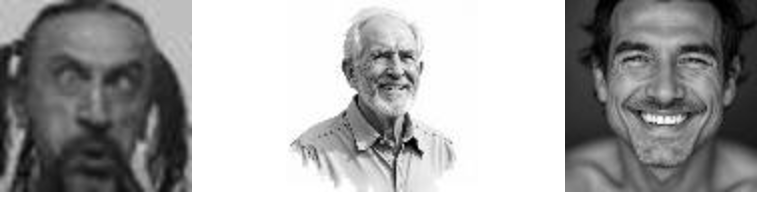
\includegraphics[width=\textwidth]{bad_annotation.png} 
    \caption{List of bad annotated photos}
    \label{fig:BadAnot}
\end{figure}

After completing all the aforementioned cleaning, filtering, and correction steps, the final dataset ready for model training stabilized at the level of 104,197 selected and normalized images.

\subsection{Exp-W Dataset Integration}
To further enrich the training corpus and improve the model's generalization capabilities, the Exp-W dataset (Cleaned version) \cite{expw} was incorporated into the project. The initial set contained 19,290 images. To maintain strict consistency with our quality standards, this supplementary dataset was subjected to the identical preprocessing pipeline:

\begin{itemize}
    \item \textbf{Deduplication (pHash \& BK-Tree):} Utilizing the perceptual hashing algorithm combined with a BK-Tree data structure for efficient similarity searching. This approach allowed for sub-linear time complexity during duplicate detection. 13 duplicate images were identified and removed.
    
    \item \textbf{Artifact Removal (EasyOCR):} The EasyOCR library was utilized to scan for text overlays. A safety threshold of 2 characters was established to avoid false positives from compression artifacts. This filter discarded 25 contaminated images.
    
    \item \textbf{Demographic Filtering (ViT-Age):} To automate the removal of images depicting children, we implemented a pre-trained Vision Transformer model (\texttt{nateraw/vit-age-classifier}). The pipeline specifically targeted the "0-2" age category (infants/toddlers). This phase reduced the dataset by 2,014 samples.
    
\begin{sloppypar}
\item \textbf{Non-photorealistic Image Removal (CLIP):} To eliminate caricatures, 3D renders, and cartoons, we employed the CLIP (\textit{Contrastive Language-Image Pre-training}) model developed by OpenAI (\texttt{clip-vit\-base\-patch32}). Using zero-shot classification, the system compared each image against two textual prompts: "a photo of a real human face" vs. "a drawing, cartoon, anime, illustration or sketch". Images with a "drawing" probability exceeding a 0.8 threshold (294 samples) were moved to the rejection folder.
\end{sloppypar}
\end{itemize}

Following this comprehensive, multi-model filtration process, 16,944 highly reliable images were successfully extracted and merged into the final database.

\section{Images generated with Flux.2}
To expand our dataset with additional images, we used generative artificial intelligence models. Our choice fell on the advanced Flux.2 [dev] \cite{flux} model, featuring 12 billion parameters. An attempt to run it in the Kaggle Notebook environment proved suboptimal — generating a single image took approximately 5 minutes. For this reason, we conducted the initial model tests through the Hugging Face platform.
The resulting images were highly consistent with the scientific definitions of individual facial expressions, as illustrated in Figure \ref{fig:emotions}. We prepared a base of 10,000 text prompts for image generation, focusing exclusively on generating human faces expressing the seven basic emotions. We also ensured that the dataset was appropriately balanced in terms of ethnic diversity. Due to the nature of the project and the intended placement of our robot's head, we restricted the generated images to children's faces aged 4 and above.
A sample input data structure is as follows: {"prompt": "headshot of sad 10 year old European boy, drooping eyelids with loss of eye focus, lips slightly pulled down at corners, grieving expression, overcast outdoor light, highly detailed, photorealistic", "emotion": "sad"}
Sample images generated using the Flux.2 [dev] model are shown in Figure \ref{fig:generated_em}.

\begin{figure}[H]
    \centering
    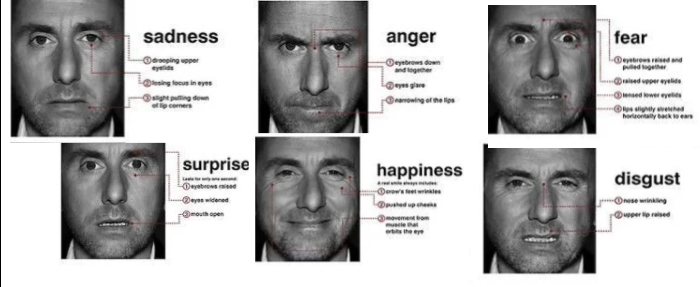
\includegraphics[width=\textwidth]{emotions.png} -
    \caption{Definition of facial emotions. Source: \href{https://pl.pinterest.com/pin/836825174527929558/}{Pinterest}}
    \label{fig:emotions}
\end{figure}

\begin{figure}[H]
	\centering
	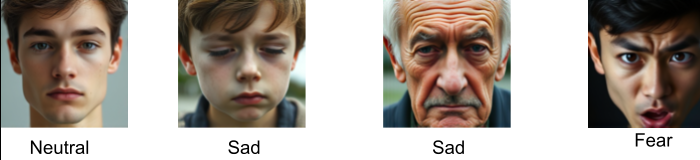
\includegraphics[width=\textwidth]{generated_em.png} 
	\caption{Examples of generated emotions with Flux.2 [dev].}
	\label{fig:generated_em}
\end{figure}

\subsection{Generation of a Synthetic Dataset}

The process of creating a synthetic dataset was divided into three stages, differing in the configuration parameters of the model (Flux.2 [dev]) and the architecture of the introduced prompts. The main assumption in all three stages was to ensure high diversity and representativeness of the dataset. For this purpose, demographic variables such as gender, age range, and ethnic origin were taken into account.

\subsubsection{Stage I: Generation Based on Scientific Definitions (10,000 images)}
In the first phase, the focus was on the rigorous reproduction of scientific definitions of facial expressions for individual emotions.

\begin{itemize}
    \item Generation parameters: Non-optimal (in terms of quality) parameter values were applied. A low number of iteration steps (15) and a low guidance scale value of 3.
    \item Results: Due to the adopted parameters, the generation of a single image was highly computationally efficient (average time: approximately 5 seconds). The obtained images (cf. Figure~\ref{fig:fluxV1}) constituted an almost perfect, textbook reflection of the emotion definitions. This resulted in an unrealistic representation of emotions, which in reality is characterized by much greater variance.
    \item Prompt structure: Prompts were constructed in a strict manner. \\
    Example: \textit{"headshot of sad 10 year old European boy, drooping eyelids with loss of eye focus, lips slightly pulled down at corners, grieving expression, overcast outdoor light, highly detailed, photorealistic"}
\end{itemize}

\begin{figure}[H]
    \centering
    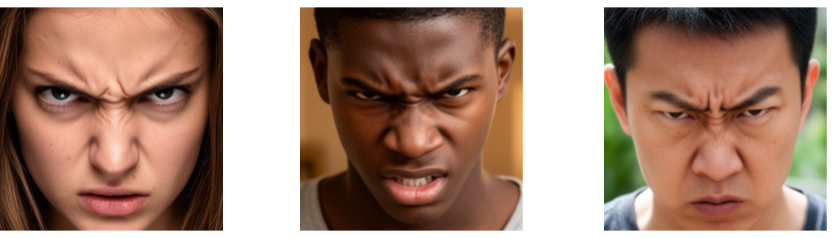
\includegraphics[width=0.45\textwidth]{flux_1.png}
    \caption{Examples pictures generated in Stage I}
    \label{fig:fluxV1}
\end{figure}

\subsubsection{Stage II: Optimization for Realism (20,000 images)}
In the second phase, strict adherence to scientific definitions was abandoned. More focus was placed on natural and varied descriptions.

\begin{itemize}
    \item Generation parameters: The efficient parameters from the first stage were maintained (15 iteration steps, guidance scale of 3; average generation time approx. 5 seconds).
    \item Results: The introduction of prompt modifications and allowing a face angle deviation of 15–20 degrees relative to the camera axis significantly increased the realism of the obtained samples (cf. Figure~\ref{fig:fluxV2}).
    \item Prompt structure: Prompts described emotions in a more realistic manner, allowing for natural expression. \\
    Example: \textit{"medium close-up portrait of a adult (30-45 years old) south asian female, showing neutral emotion with blank gaze, context: listening, harsh overhead light, plain gray background, face clearly visible, realistic facial expression, candid photograph, natural expression"}
\end{itemize}

\begin{figure}[H]
    \centering
    \includegraphics[width=0.45\textwidth]{flux_2.png}
    \caption{Examples pictures generated in Stage II}
    \label{fig:fluxV2}
\end{figure}

\subsubsection{Stage III: High-Quality Generation (17,600 images)}
The third phase was an extension of the assumptions from Stage II, with particular emphasis on maximizing visual quality and the introduction of advanced variability in lighting conditions.

\begin{itemize}
    \item Generation parameters: The computational load was significantly increased by setting the maximum number of iteration steps to 50 and raising the guidance scale to a level of 6 (on a 10-point scale).
    \item Results: The effect of changing the parameters was obtaining images of the highest detail, characterized by high realism (cf. Figure~\ref{fig:fluxV3}). However, the increase in precision was associated with a significant drop in efficiency – the average generation time increased to approx. 33 seconds per image.
    \item Prompt structure: Prompts were highly elaborate, incorporating dynamic head positioning and lighting descriptions. \\
    Example: \textit{"slight 3/4 angle portrait of a mid 30s indigenous american person, braided hair, with a scar on cheek, displaying fearful — frozen deer-in-headlights stare, situation: receiving emergency news, ring light, blurred bokeh city lights background, sun-kissed skin, face fully visible and in sharp focus, authentic human facial expression, high-resolution 8k portrait, ultra-sharp details"}
\end{itemize}

\begin{figure}[H]
    \centering
    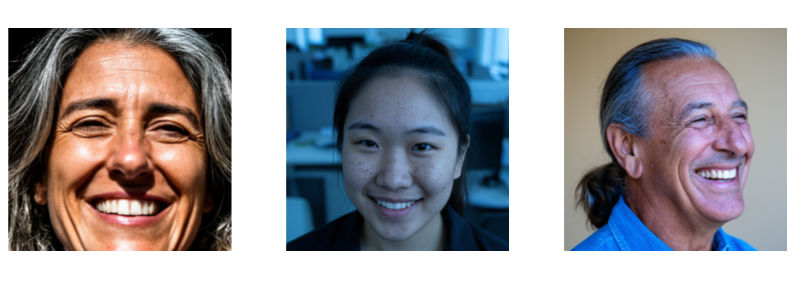
\includegraphics[width=0.45\textwidth]{flux_3.png}
    \caption{Examples pictures generated in Stage III}
    \label{fig:fluxV3}
\end{figure}

\subsection{Flux Models Detailed Training Analysis}

\begin{figure}[H]
	\centering
	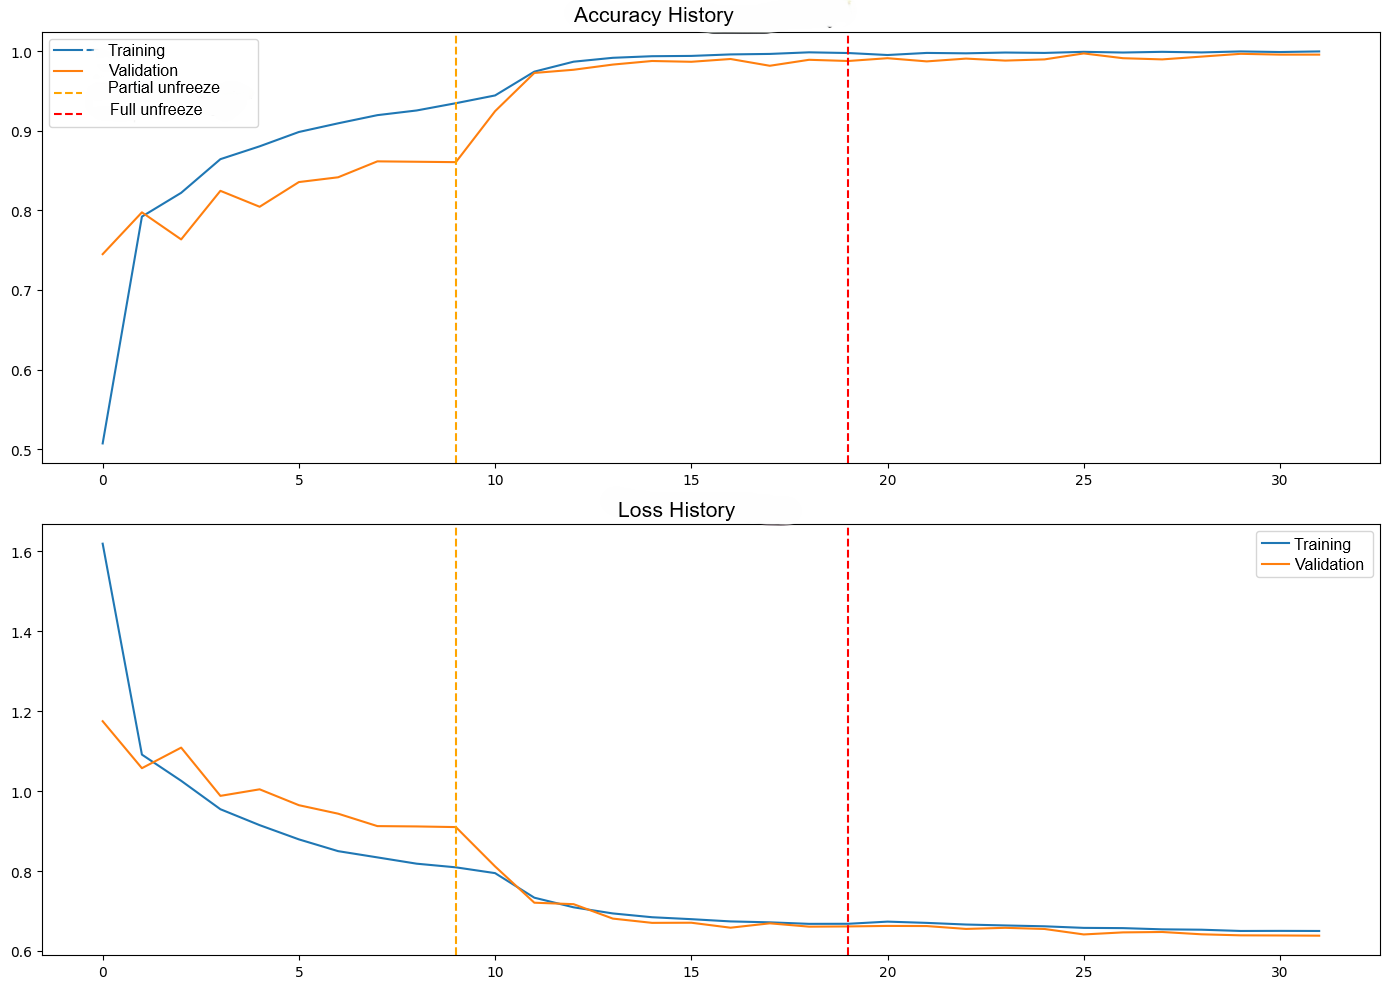
\includegraphics[width=0.45\textwidth]{flux1_history.png}
	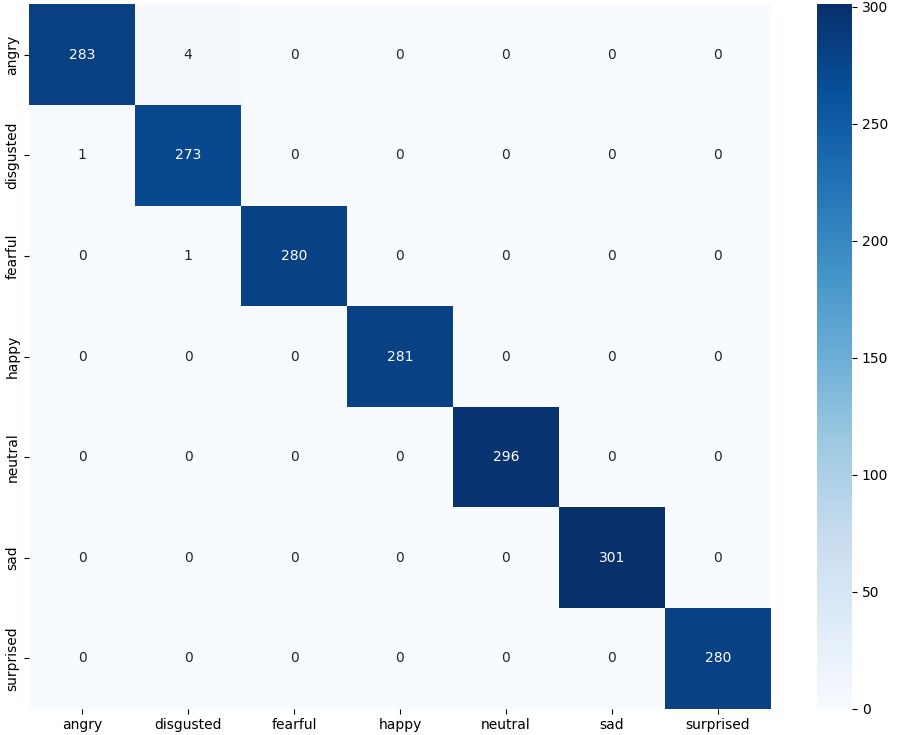
\includegraphics[width=0.45\textwidth]{flux1_cm.png}
	\caption{Metrics for Dataset 1 Evidence of extreme overfitting to specific prompts.}
	\label{fig:flux_run1}
\end{figure}

\begin{figure}[H]
	\centering
	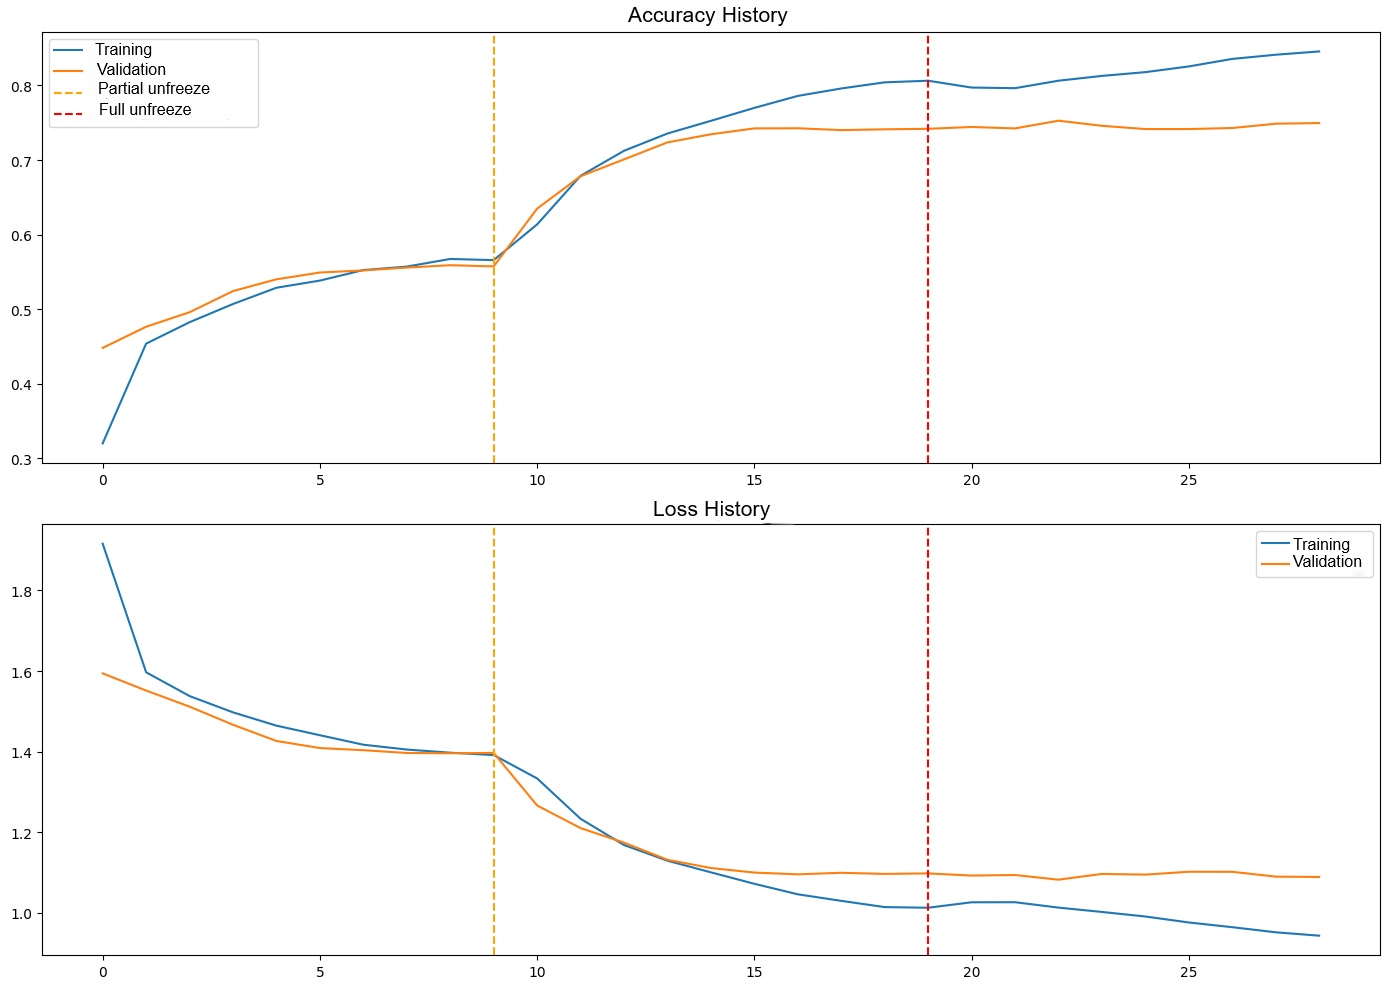
\includegraphics[width=0.45\textwidth]{flux2_history.png}
	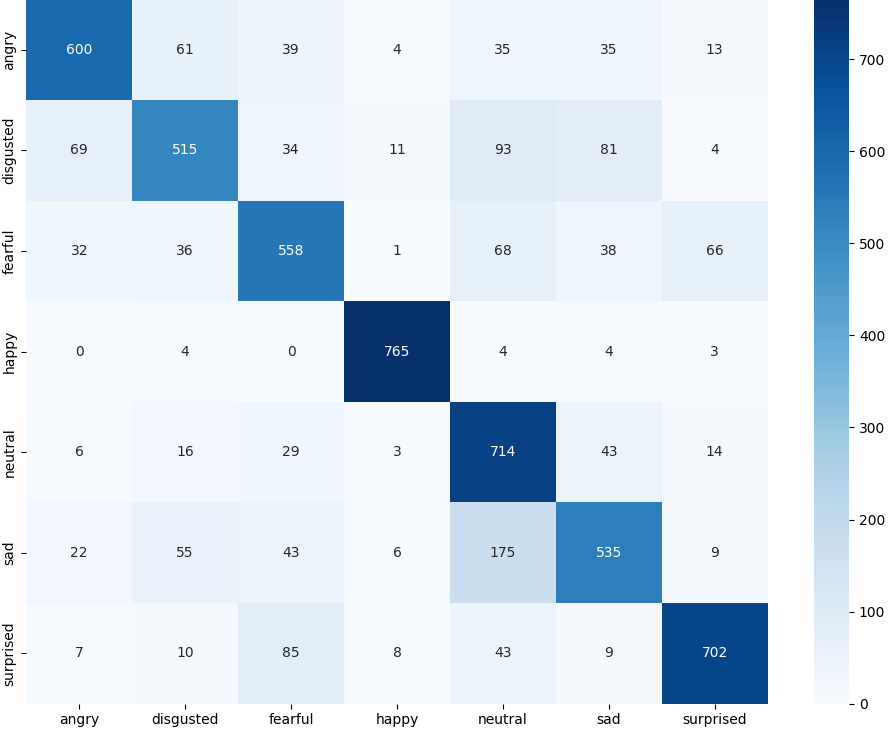
\includegraphics[width=0.45\textwidth]{flux2_cm.png}
	\caption{Metrics for Dataset 2 Balanced training with realistic generalization.}
	\label{fig:flux_run2}
\end{figure}

\begin{figure}[H]
	\centering
	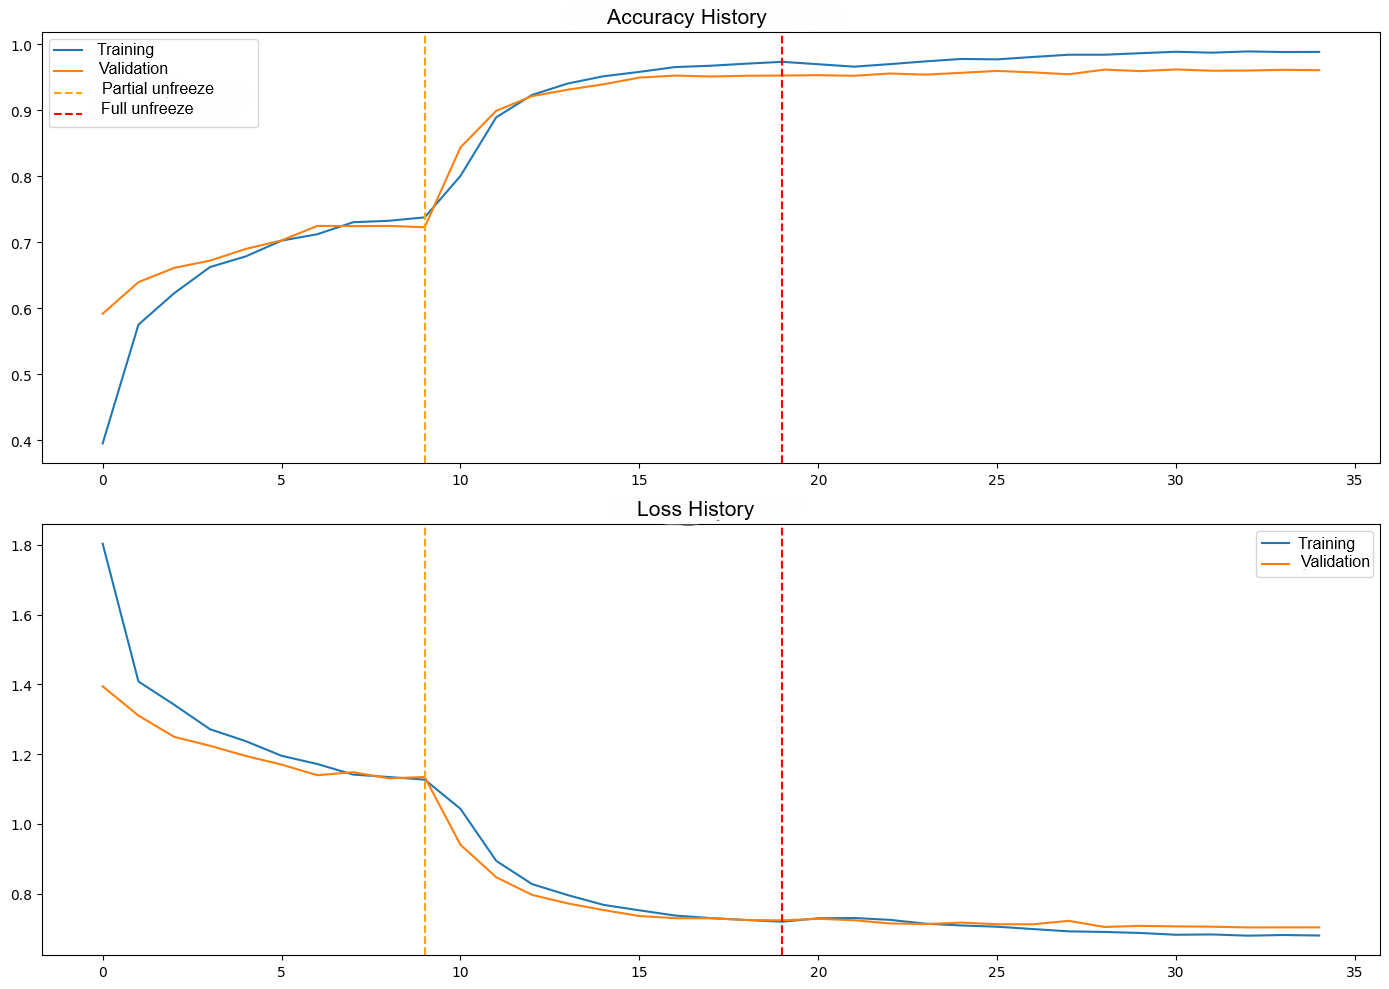
\includegraphics[width=0.45\textwidth]{flux3_history.png}
	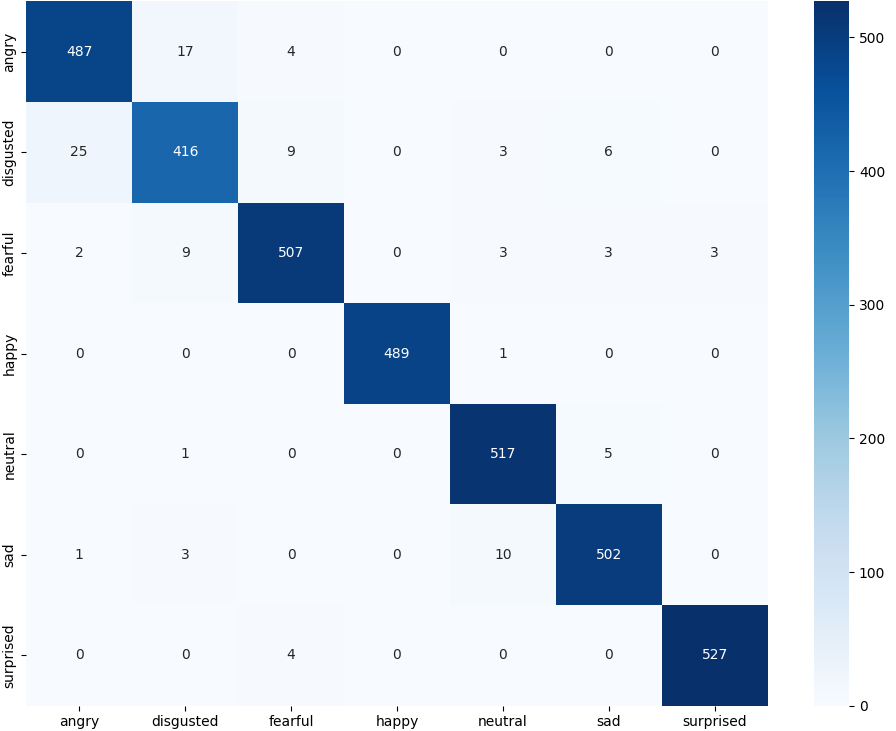
\includegraphics[width=0.45\textwidth]{flux3_cm.png}
	\caption{Metrics for Dataset 3 High validation scores masking poor practical utility.}
	\label{fig:flux_run3}
\end{figure}

The evaluation of synthetic data impact was performed using three distinct datasets generated by the FLUX.2 dev model. Each dataset consists of a different number of images generated using unique prompt strategies. Dataset 1 contains 10000 images. Dataset 2 contains 20000 images. Dataset 3 contains 17600 images. The exact prompt formulas and generation details for each set will be described in the following sections. The metrics achieved for each unique dataset are presented in the table below.

\begin{table}[H]
	\centering
	\begin{tabular}{|l|c|c|c|c|}
		\hline
		\textbf{Dataset Variant} & \textbf{Accuracy} & \textbf{Precision} & \textbf{Recall} & \textbf{F1 Macro} \\ \hline
		Flux Dataset 1 & 99.70\% & 0.9969 & 0.9969 & 0.9969 \\ \hline
		Flux Dataset 2 & 76.90\% & 0.7764 & 0.7701 & 0.7694 \\ \hline
		Flux Dataset 3 & 96.93\% & 0.9687 & 0.9684 & 0.9685 \\ \hline
	\end{tabular}
	\caption{Performance metrics for models trained on three distinct FLUX.1 datasets.}
	\label{tab:flux_all_results}
\end{table}

The extreme performance gap between the datasets highlights a critical issue in using synthetic data for emotion recognition. While Dataset 1 and Dataset 3 show nearly perfect accuracy, these results are deceptive and do not translate to practical performance. During live camera testing, models trained on these sets failed to identify expressions on real human faces. This is a clear case of the network overfitting to specific digital artifacts and the consistent idealized nature of the prompts used in those versions. The models effectively memorized the synthetic patterns instead of learning universal human facial features.

In contrast, Dataset 2 was generated using more complex and noisy prompts, including various lighting conditions and subtle expression changes. Although the accuracy is lower at 76.90\%, this model proved to be the only one with genuine generalization capabilities. It successfully recognizes emotions in live interactions, confirming that a lower validation score on synthetic data can often indicate a more robust model for practical deployment.

\subsection{Alternative Attempt with Hunyuan Image 3}
After successfully generating images with the Flux model we decided to test other available generative architectures. We attempted to use the quantized Hunyuan Image 3 model in the NF4 format. The experiments were conducted on the departmental server which is equipped with two NVIDIA graphics cards each possessing 48 GB of VRAM. Despite having 96 GB of total video memory the generation process encountered critical architectural limitations. The primary issue was the inability of the PyTorch environment to properly distribute the model weights across both GPUs. Using automatic memory balancing resulted in CUDA out of bounds errors during the attention mechanism calculations. Attempting to manually assign the neural network layers to specific cards caused communication failures between the tokenizer and the main model. The system failed to generate even a single image returning only execution errors. Due to these numerous and persistent hardware communication problems we completely abandoned the use of this model.

\section{Final training dataset}
After combining the rigorously cleaned baseline dataset (104,197 images) with the processed Exp-W samples (16,944 images), the final unified dataset ready for model training reached a total volume of 121,133 normalized images.

\section{Convolutional neural networks}
\begin{quote}
Convolutional neural networks (CNNs) are the most prominent type of AI algorithm for image processing out there today. Put simply, a CNN takes a visual input (a digital image) and applies a series of filter operations to that input. Through this process, a certain type of information or output is extracted from the input image. This could, for example, be the type of object that is displayed in the input (a.k.a. image classification), but it could also be a partitioning of the input into different regions (a.k.a. image segmentation) or something else entirely. CNNs are very versatile in that respect and can be used to solve all kinds of image processing problems. For those interested in analogies with biology, think of the way that the visual cortex processes information (cf. works of Hubel \& Wiesel) – CNNs are inspired by and closely related to this architecture.\footnote{Mateusz Miłosz, \textit{Convolutional Neural Networks Demystified: How Immunofluorescence Images Are Processed in Modern Labs}. Available at: \href{https://www.euroimmun.pl/splotowe-sieci-neuronowe-bez-tajemnic-jak-przetwarza-sie-obrazy-immunofluorscencyjne-w-nowoczesnych-laboratoriach/?post_language=en}{[Link to the article]}}
\begin{figure}[h]
    \centering
    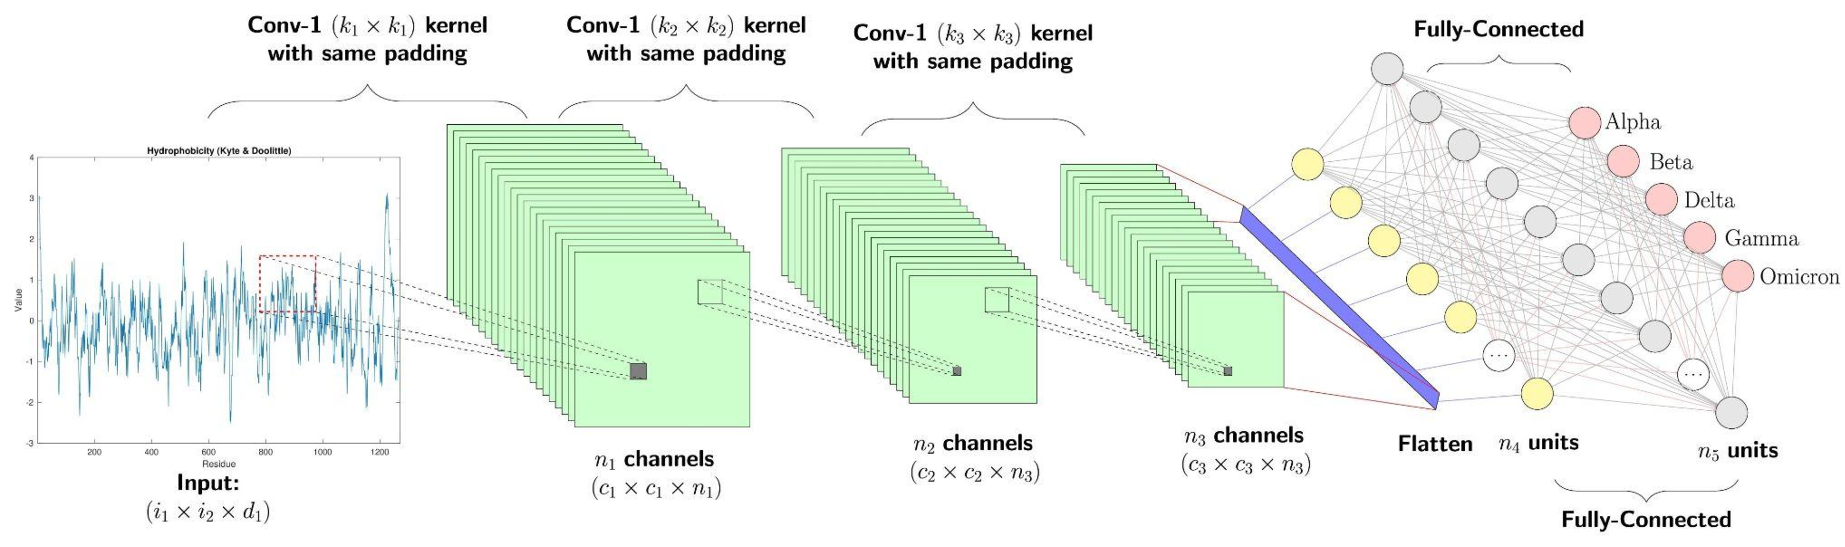
\includegraphics[width=\textwidth]{CNN.png} 
    \caption{CNN network example}
    \label{fig:CNN}
\end{figure}

\end{quote}
\subsection{Literature Review and Theoretical Foundation}
The development of an original neural network architecture was preceded by a thorough review of the relevant literature and scientific publications in the field of human emotion recognition using Convolutional Neural Networks (CNNs). Knowledge regarding the operational mechanisms of convolutional networks and the functions of individual model layers was systematized based on the official technical documentation of the TensorFlow \cite{tensorflow} library and specialist educational materials (including the GeeksforGeeks portal\footnote{shibsankar saw, \textit{Emotion Detection Using Convolutional Neural Networks (CNNs)}. Available at: \href{https://www.geeksforgeeks.org/deep-learning/emotion-detection-using-convolutional-neural-networks-cnns/}{[Link to the article]}}).
The following technology stack was employed in the process of designing and implementing the system:
\begin{itemize}
\item TensorFlow — The selection of this framework was driven by its high performance and streamlined deployment process for trained models on embedded platforms. This aspect was of critical importance due to the intended implementation of the system on a Raspberry Pi microcomputer.
\item TensorBoard — This tool was implemented for the purpose of monitoring and evaluating model metrics. It enables real-time logging of parameters during the training process and their visualization within a dedicated graphical interface, while offering advanced filtering and data view customization capabilities.
\item TensorFlow Keras (tf.keras) — This module was used to optimize dataset management. It facilitated the partitioning of the available corpus into training, validation, and test sets, in proportions of 70 percent 20 percent  10 percent respectively. Furthermore, due to significant class imbalance within the dataset (a considerably smaller number of samples for selected emotion categories), the library's mechanisms were employed to analytically compute and assign weights to individual classes, thereby preventing the model from exhibiting a bias toward dominant classes.
\item Scikit-learn (sklearn) — This library was utilized primarily for the generation of a confusion matrix. It constitutes a fundamental analytical tool within the project, enabling detailed evaluation of classifier performance and assessment of prediction accuracy across individual emotion categories.
\end{itemize}

\subsection{Problems encountered}
\subsubsection{Environmental Challenges and Hardware Resource Optimization}
During the implementation phase of the neural network model, several critical issues of an environmental and hardware nature were identified. The main obstacle was the lack of native GPU acceleration support on Windows for the TensorFlow library (version 2.11 and later). This problem was resolved by migrating the runtime environment to the WSL2 subsystem (Windows Subsystem for Linux).
A further challenge was the aggressive allocation of all available GPU VRAM by TensorFlow processes, which led to system instability. This issue was mitigated at the algorithm code level by enabling dynamic memory management (memory growth). As a result, only the amount of VRAM strictly necessary for efficient computation at any given moment is allocated to the network training process.
\subsubsection{ Overfitting and the Model Checkpointing Mechanism}
During training runs on various datasets, it was observed that models tend to overfit very rapidly. The critical point at which the model's generalization capability began to deteriorate sharply typically occurred between the 8th and 11th epoch.
To prevent the loss of the best network weights, a Model Checkpointing mechanism was implemented. The algorithm was configured to permanently save the model state only during those epochs in which the validation loss reaches a value lower than in previous iterations.
\subsubsection{Analysis of the Root Causes of Early Overfitting}
The rapid degradation of validation results and the aggressive overfitting observed in the trained models stems from the convergence of several factors, related primarily to the quality and characteristics of the input data:
\begin{itemize}
    \item Memorization - Rather than extracting universal features, a model with high parameter capacity begins to "memorize" specific images from the training set. This results in high accuracy on training data and a drastic drop in performance on new, previously unseen images.
    \item Noisy Labels - The datasets used frequently contain low-quality images ("garbage" data) or carry incorrectly assigned labels (e.g., a neutral face labeled as sad). The network's attempt to fit such anomalies forces it to develop false, overly complex decision rules, which directly accelerates the overfitting process.
    \item Insufficient Data Diversity - A lack of adequate variance in the training set causes the model to quickly exhaust the pool of available features. In such cases, the application of strong regularization and Data Augmentation techniques becomes essential.
\end{itemize}

\subsection{First simple model}
The designed architecture constitutes a classical deep convolutional neural network (CNN), optimized for the extraction of spatial features from facial images and the classification of emotional states. The model was built in a layered fashion, with a clear division into a feature extraction module and a final element serving as the classifier.
\subsubsection{Code review}
\begin{lstlisting}
def first_model():
    inputs = Input(Input_shape)

    conv1 = layers.Conv2D(32, (3, 3), strides=(1, 1), kernel_regularizer=l2(0.001))(inputs)
    conv1 = layers.Dropout(0.1)(conv1)
    conv1 = layers.Activation('relu')(conv1)
    pool1 = layers.MaxPooling2D((2, 2))(conv1)

    conv2 = layers.Conv2D(64, (3, 3), strides=(1, 1), kernel_regularizer=l2(0.001))(pool1)
    conv2 = layers.Dropout(0.1)(conv2)
    conv2 = layers.Activation('relu')(conv2)
    pool2 = layers.MaxPooling2D((2, 2))(conv2)

    conv3 = layers.Conv2D(128, (3, 3), strides=(1, 1), kernel_regularizer=l2(0.001))(pool2)
    conv3 = layers.Dropout(0.1)(conv3)
    conv3 = layers.Activation('relu')(conv3)
    pool3 = layers.MaxPooling2D((2, 2))(conv3)

    conv4 = layers.Conv2D(256, (3, 3), strides=(1, 1), kernel_regularizer=l2(0.001))(pool3)
    conv4 = layers.Dropout(0.1)(conv4)
    conv4 = layers.Activation('relu')(conv4)
    pool4 = layers.MaxPooling2D((2, 2))(conv4)

    # Classifier
    flatten = layers.Flatten()(pool4)
    dense = layers.Dense(128, activation='relu')(flatten)
    drop_1 = layers.Dropout(0.2)(dense)
    outputs = layers.Dense(num_emotions, activation='softmax')(drop_1)

    model = Model(inputs=inputs, outputs=outputs, name="first_model")
    model.summary()
    return model
\end{lstlisting}
\begin{itemize}
    \item \texttt{layers.Conv2D(32, (3, 3), strides=(1, 1), kernel\_regularizer=l2(0.001))} \\
    This is a two-dimensional convolutional layer responsible for extracting features from facial images. It slides 32 different filters of size 3x3 (kernel) across the entire image one pixel at a time (\texttt{strides=(1,1)}), searching for edges, curves, and specific textures. The \texttt{kernel\_regularizer=l2} parameter adds a penalty to the loss function for excessively large weight values, which is a technique used to prevent model overfitting.
    
    \item \texttt{layers.Dropout(0.1)} \\
    A regularization layer that randomly "switches off" (zeroes out) a specified fraction of neurons (in this case, 10\%) during each training step. This forces the network to develop more generalized patterns and prevents overfitting to specific images in the training set.
    
    \item \texttt{layers.Activation('relu')} \\
    Defines the ReLU (Rectified Linear Unit) activation function. Its role is to introduce non-linearity into the model by zeroing out all negative values while passing positive values through unchanged. This enables the network to learn complex, non-linear relationships.
    
    \item \texttt{layers.MaxPooling2D((2, 2))} \\
    A pooling layer that reduces the spatial resolution of the feature map by half. It selects the highest value from each 2x2 pixel region. This drastically reduces the number of parameters to be computed and makes the model less sensitive to minor shifts of the face within the frame.
    
    \item \texttt{layers.Flatten()} \\
    A flattening layer. It takes the three-dimensional feature maps generated by the preceding convolutional layers and reshapes them into a one-dimensional vector. This is a necessary step in order to pass the extracted features to a classical dense network (the classifier).
    
    \item \texttt{layers.Dense(128, activation='relu')} \\
    A fully connected dense layer (every neuron is connected to every neuron in the preceding layer). It acts as the primary classifier, making decisions based on the flattened feature vector that lead to emotion recognition. It contains 128 neurons and its own ReLU activation function.
    
    \item \texttt{activation='softmax'} \\
    An activation function used in the final (output) layer of the network for multi-class problems. It transforms the network's raw numerical outputs into a probability distribution — as a result, the output values always sum to 1.0 (100\%).
    
    \item \texttt{model = Model(inputs=inputs, outputs=outputs, name="first\_model")} \\
    A function from the Keras Functional API that physically creates the model object. It connects the previously defined data entry point (\texttt{inputs}) with the final layer (\texttt{outputs}) into a single graph structure, which can then be compiled, trained (by calling the \texttt{.fit()} method), and used for inference.
\end{itemize}

\subsubsection{Training metrics}
The neural network training process was carried out using a dataset comprising 104,197 grayscale images with a standardized resolution of 96×96 pixels. At this stage of experimentation, data augmentation techniques were deliberately omitted in order to establish the model's baseline generalization capability. As a result, upon completion of the training process, a validation accuracy of approximately 63\% was achieved.
The computational experiments were conducted in a local environment (a mobile workstation), utilizing the Windows Subsystem for Linux (WSL2) architecture to ensure framework compatibility with hardware acceleration. The hardware platform used for training had the following specification:
\begin{itemize}
    \item CPU - Intel Core i9 13th Generation (base clock 2.20 GHz)
    \item RAM - 16 GB DDR5 (5600 MHz, CL46 latency)
    \item GPU - NVIDIA GeForce RTX 4060 with 8 GB dedicated VRAM
\end{itemize}
Based on the conducted training, we generated the confusion matrix shown in Figure \ref{fig:cmfirst}.
 
\begin{figure}[H]
    \centering
   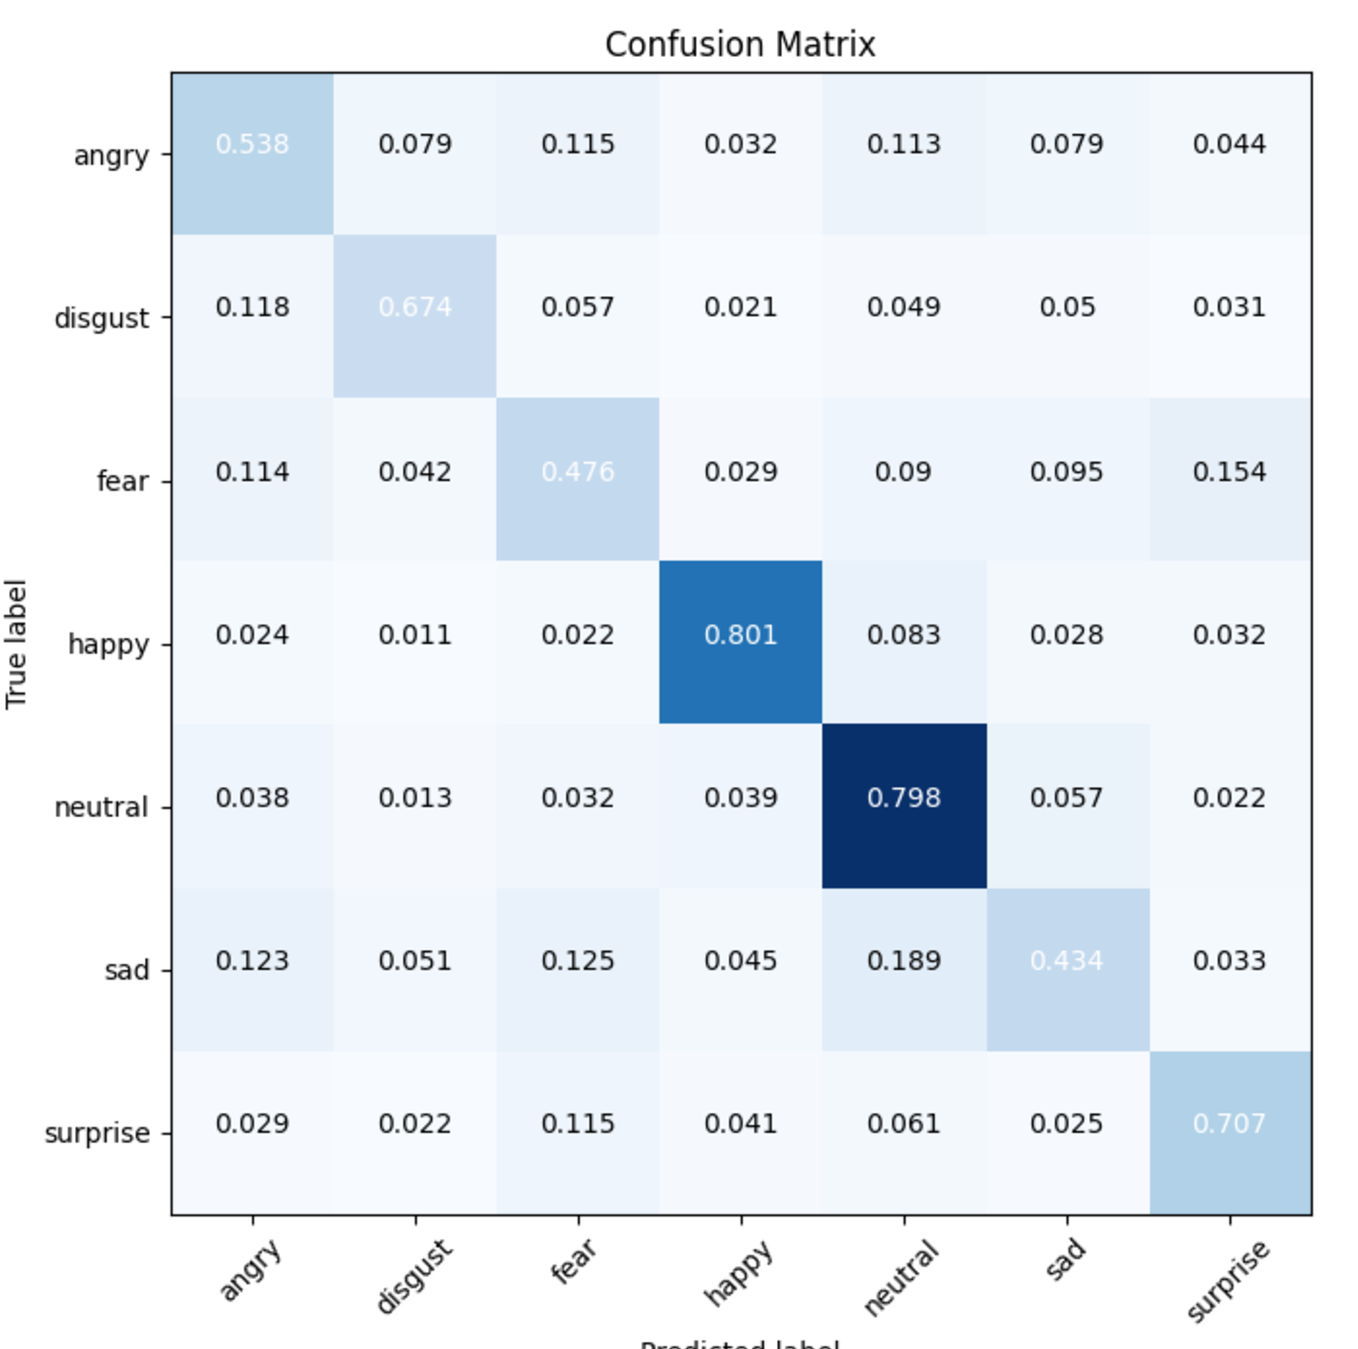
\includegraphics[width=\textwidth]{cm_first.png} 
    \caption{Confusion matrix}
    \label{fig:cmfirst}
\end{figure}

\begin{itemize}
    \item Accuracy 
    \begin{align*}
        \text{Accuracy} &= \frac{TP+TN}{TP+TN+FP+FN} \\&= \frac{0.538 + 0.674 + 0.476 + 0.801 + 0.798 + 0.434 + 0.707}{7} \\
        &\approx 0.6326 \ (63.26\%)
    \end{align*}

    \item Precision 
    \begin{align*}
        \text{Precision}_{\text{happy}} &= \frac{TP}{TP + FP} \\
        &= \frac{0.801}{0.032 + 0.021 + 0.029 + 0.801 + 0.039 + 0.045 + 0.041} \\
        &= \frac{0.801}{1.008} \approx 0.7946 \ (79.46\%)
    \end{align*}
\end{itemize}
Analysis of the loss function curves for the training and validation sets (Figure \ref{fig:lossfirst}) reveals clear symptoms of network overfitting. The rapid degradation of validation results, observable around the 10th epoch, indicates a loss of the model's generalization capability. Furthermore, as early as the 4th epoch, a significant flattening of the validation loss curve can be observed, while the training loss continues to decrease. This points to a high likelihood of memorization, in which the model, rather than extracting universal facial expression patterns, begins to overfit to the specific characteristics of individual images in the training set.
To mitigate this issue and improve the network's performance, the following optimization steps have been planned for subsequent stages of the work:
\begin{itemize}
    \item Data Cleaning - A detailed review of the datasets will be conducted with respect to the correctness of annotations. Images of extremely low quality, those not depicting faces, or those carrying incorrect labels (noisy data) will be removed from the training process.
    \item Data Augmentation - The impact of random geometric and photometric image transformations applied in real time (e.g., rotations, brightness adjustments) on suppressing overfitting and improving the model's final evaluation metrics will be investigated.
\end{itemize}

\begin{figure}[H]
    \centering
    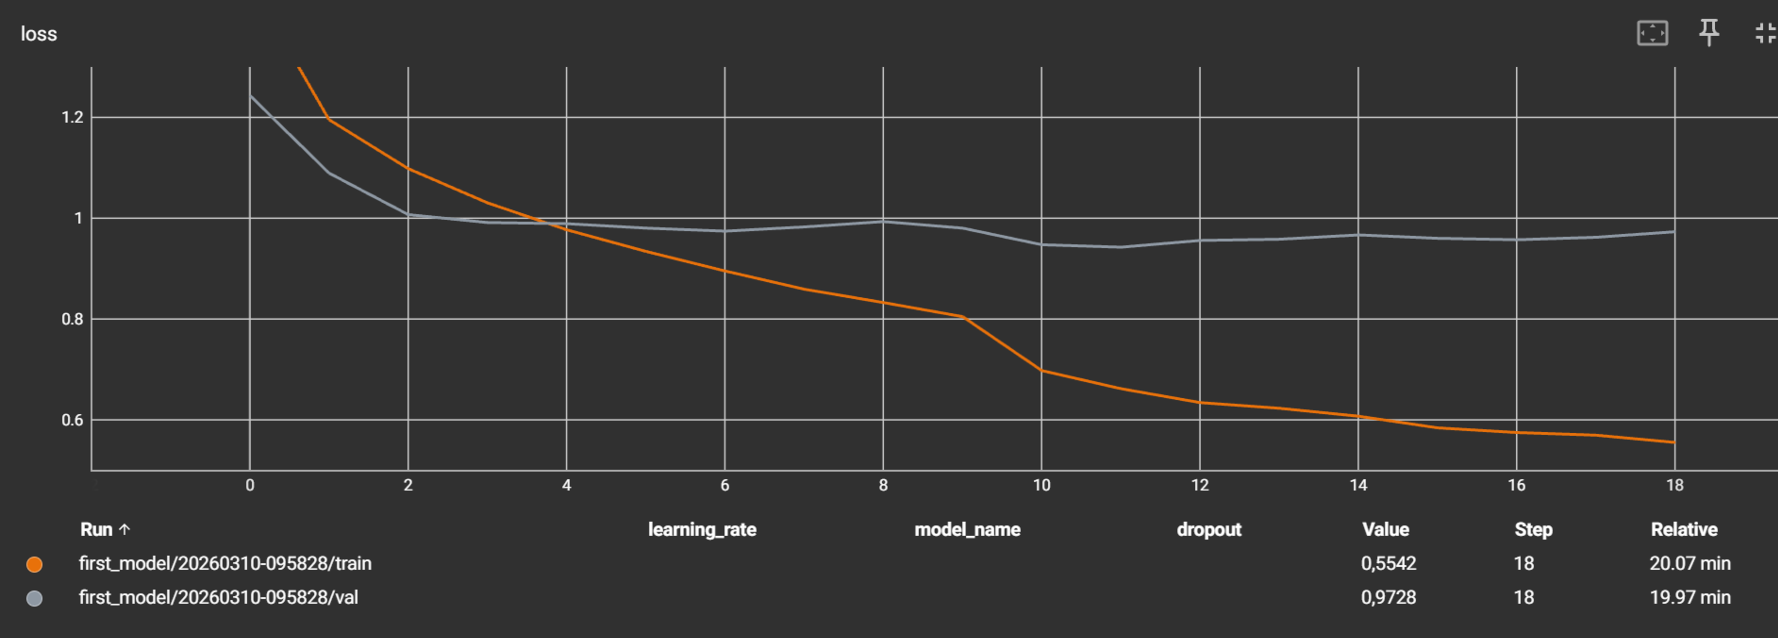
\includegraphics[width=\textwidth]{Loss_first.png} 
    \caption{Graph of validation and training loss}
    \label{fig:lossfirst}
\end{figure}


\subsection{Extended base model}
Following the baseline observations from the first model, we developed more complex custom architectures: \texttt{second\_model} and \texttt{third\_model}. These models introduced deeper feature extraction blocks and more aggressive dropout rates to counter the previously observed overfitting. 

The \texttt{second\_model} emerged as the most successful architecture in our entire study. It achieved an impressive validation accuracy of \textbf{71.04\%}. As shown in its confusion matrix (Figure \ref{fig:cm_second}), it performs exceptionally well in recognizing the "happy" emotion (over 2000 correct predictions), though it still faces challenges distinguishing between "sad" and "neutral" states. The \texttt{third\_model} also provided solid results (\textbf{67.81\%} accuracy), but exhibited slightly more instability during the validation phases.

\begin{figure}[H]
    \centering
    \begin{minipage}{0.48\textwidth}
        \centering
        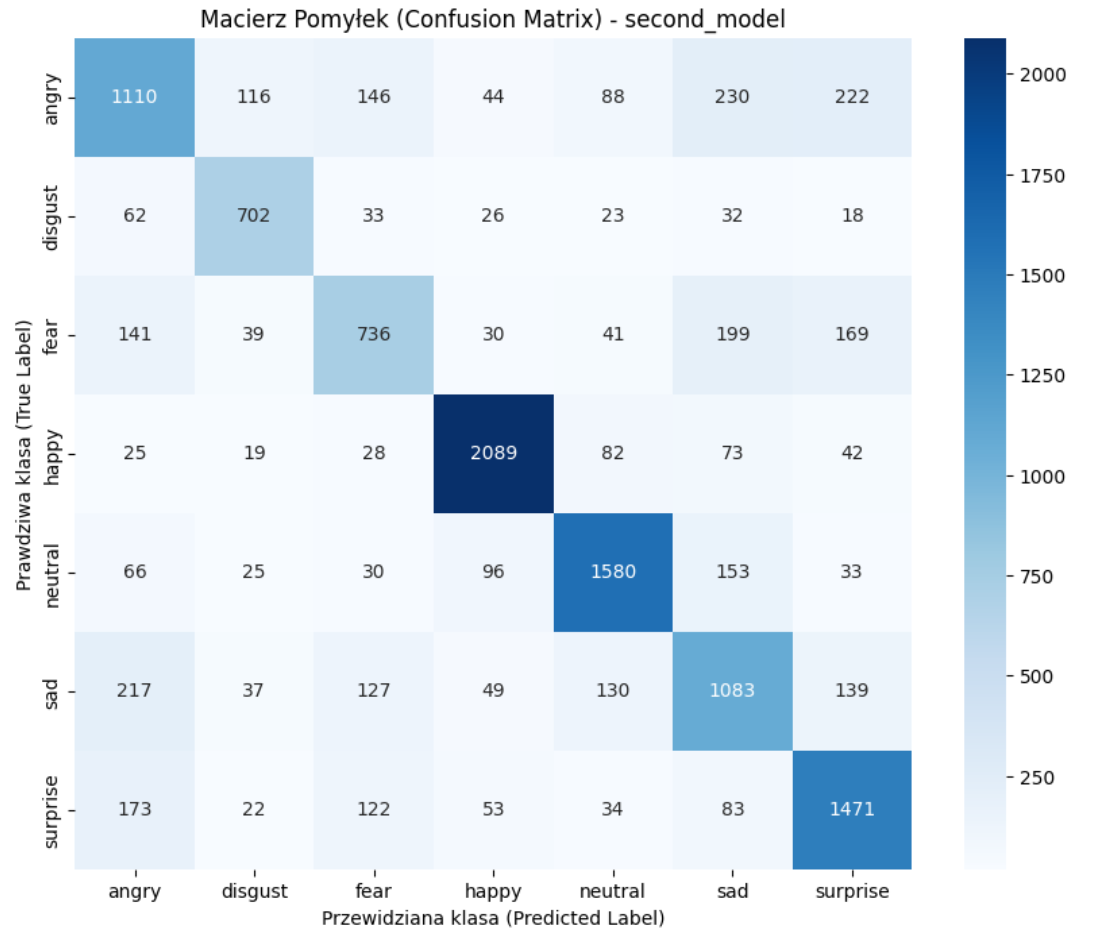
\includegraphics[width=\linewidth]{First_model_CM.png} % Plik wgrany jako First_model_CM.png dla second_model
        \caption{Confusion Matrix - second\_model}
        \label{fig:cm_second}
    \end{minipage}\hfill
    \begin{minipage}{0.48\textwidth}
        \centering
        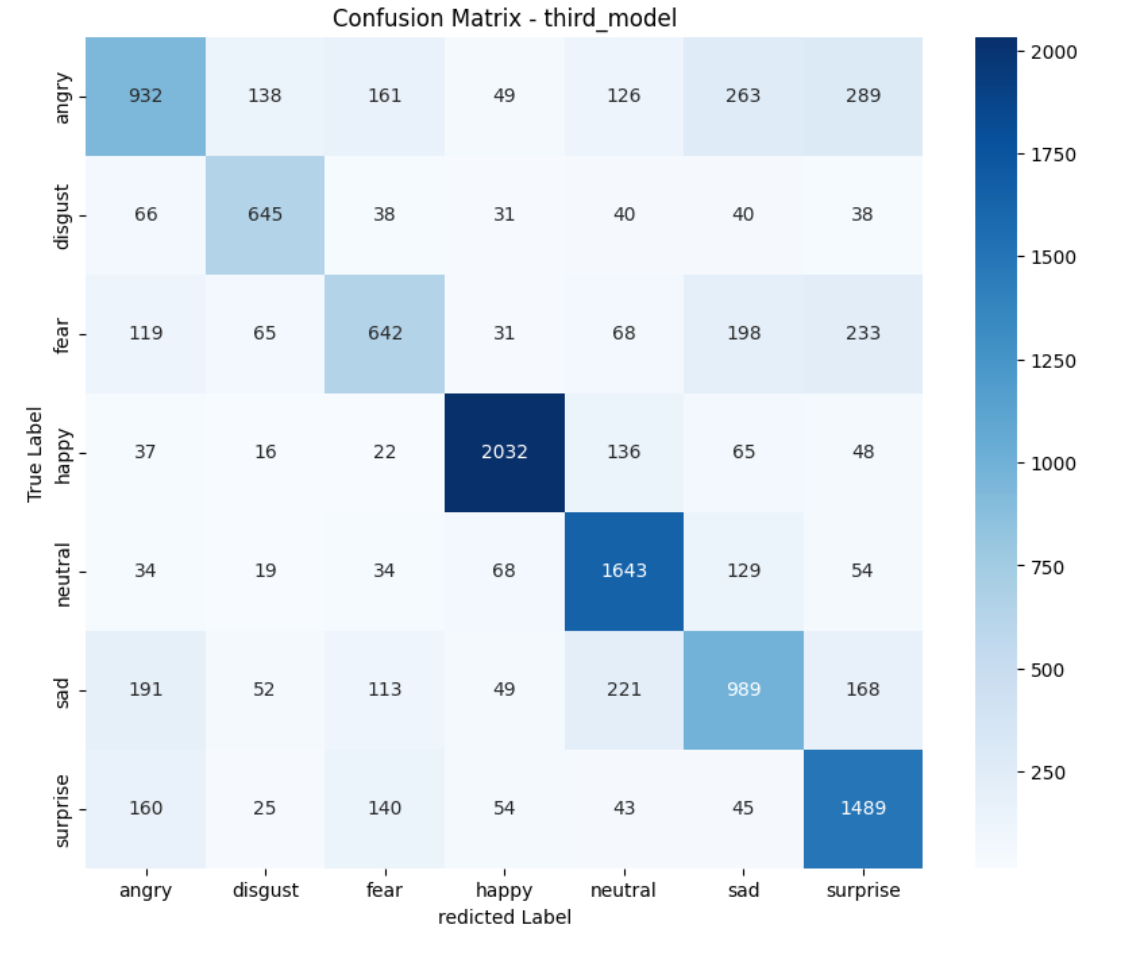
\includegraphics[width=\linewidth]{Third_model_CM.png}
        \caption{Confusion Matrix - third\_model}
        \label{fig:cm_third}
    \end{minipage}
    \label{fig:cm_second_third}
\end{figure}

The training dynamics of the \texttt{third\_model} can be observed in Figure \ref{fig:loss_third}, where the stabilization of the validation loss curve indicates a significant reduction in the memorization problem that plagued the initial basic model.

\begin{figure}[H]
    \centering
    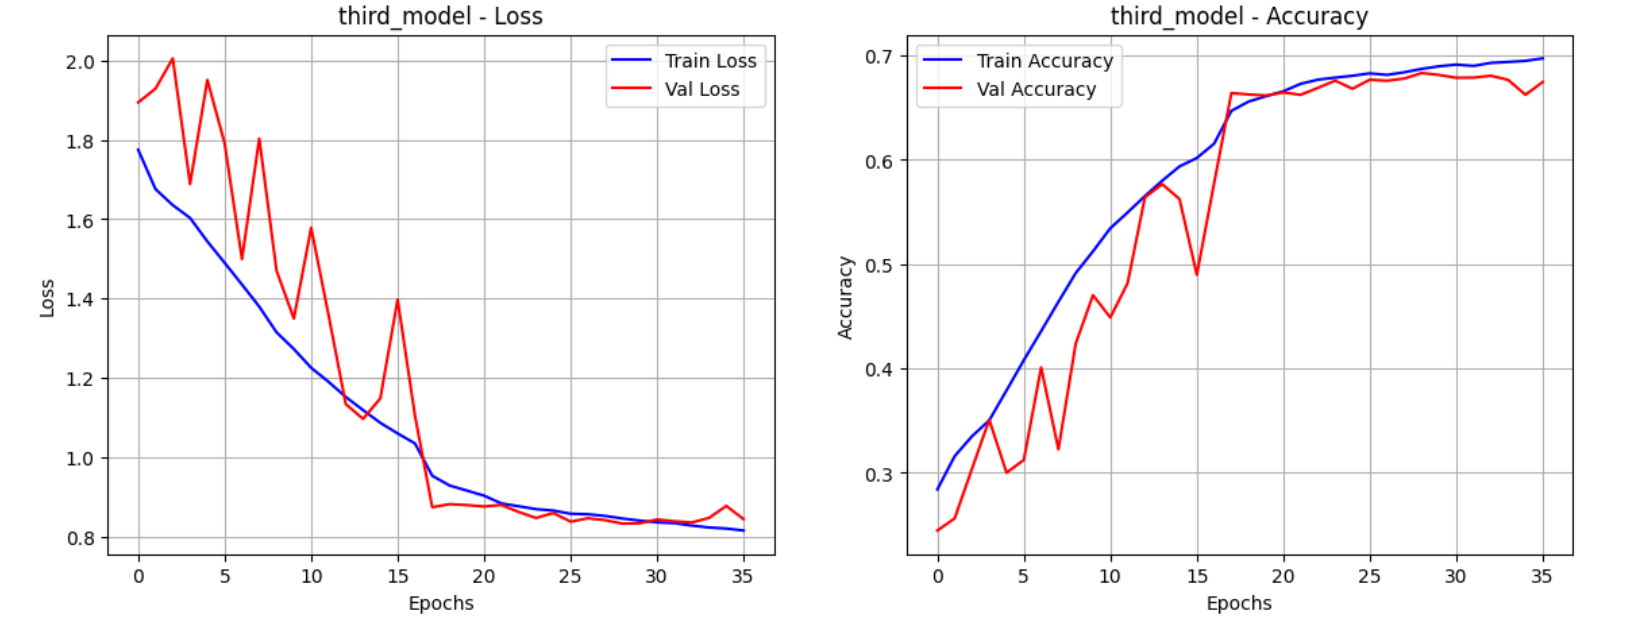
\includegraphics[width=0.8\textwidth]{Third_model.png} 
    \caption{Graph of validation and training loss/accuracy for third\_model}
    \label{fig:loss_third}
\end{figure}

\section{Comparison with reference DCNN models}
\label{sec:cnn_models}
We decided to compare the results of our best model against ready-made, pre-trained deep convolutional neural network (DCNN) models designed for image classification. For the comparison, we selected the following architectures: InceptionV3\cite{inceptionv3}, Xception\cite{xception}, ResNet50\cite{resnet}, ResNet101\cite{resnet}, VGG16\cite{vgg}, and VGG19\cite{vgg}.

\begin{itemize}
    \item The VGG family (VGG16 and VGG19): These networks were designed in 2014 by the Visual Geometry Group at the University of Oxford, in preparation for the prestigious ILSVRC competition. The variants used in the study differ from each other solely in structural depth, consisting of 16 and 19 layers respectively.
    \item The ResNet family (ResNet50 and ResNet101): Residual networks whose names directly indicate the total number of implemented layers (50 and 101). Their fundamental architectural innovation is the introduction of skip (shortcut) connections. This mechanism effectively prevents the vanishing gradient problem, enables feature transfer from the early stages of the network, and significantly improves the stability and efficiency of the training process.
    \item The InceptionV3 and Xception architectures: These are advanced models developed by Google engineers, representing a technological evolution of the classic Inception network from 2014. InceptionV3, introduced a year later, is characterized by a very extensive structure comprising 159 layers. Meanwhile, the Xception architecture, presented in 2016, bases its key feature extraction module on 36 layers.
\end{itemize}
\subsection{Fine-Tuning}
For the pre-trained models, we also applied the fine-tuning method. This process involves adapting a ready-made machine learning model to a specific task or new data that differs from the dataset used during the network's original training. Instead of training the model entirely from scratch, the 'knowledge' it has already acquired regarding the detection of universal visual features — such as edges, gradients, or basic geometric shapes — is leveraged. The fine-tuning strategy we implemented was based on the following assumptions:
\begin{itemize}
    \item Partial unfreezing of deep layers - Rather than updating weights across the entire network, we unlocked only the last 20\% of the base model's layers for training, leaving the initial 80\% permanently frozen. This is because the early layers of a convolutional network are responsible for extracting universal image features, which we do not want to modify. The final layers, on the other hand, learn high-level features specific to a given problem — which is precisely why we fine-tuned them to recognize the nuances of facial expressions.
    \item Learning rate reduction - Prior to commencing the actual fine-tuning, the model was recompiled with a learning rate ten times smaller than the default. Using the initial default value of this hyperparameter could result in overly aggressive weight updates and irreversibly destroy useful representations learned on the ImageNet dataset. A reduced learning rate allows for safe and subtle weight adjustments.
  \item Preserving training continuity -  By setting the \texttt{initial\_epoch=history.epoch[-1]} parameter, we ensured that the model resumes training from exactly the epoch at which the initial (warm-up) phase ended. This guarantees logical and numerical continuity throughout the entire learning process.
\end{itemize}

\subsection{Problems with datasets}
A significant issue during evaluation turned out to be the format of the input data. The DCNN models listed in section \ref{sec:cnn_models} are by design adapted to process three-channel color images (RGB) at a resolution of 224x224 pixels. Our existing training dataset, however, consisted of grayscale images at a resolution of 96x96 pixels. This difference significantly affected the initial results. After launching the preliminary training on the InceptionV3 model, accuracy stalled at around 40\% after just a few epochs, as illustrated in the chart below. This chart presents both the pre-training phase and the metrics obtained during the fine-tuning stage. As can be observed, fine-tuning ultimately made it possible to surpass the 60\% accuracy threshold. However, bearing in mind the architectural requirements of the pre-built networks, we made the decision to convert the entire dataset from grayscale to the RGB color space, combined with an artificial colorization process (details are described in section \ref{sec:colorization}).

\begin{figure}[H]
    \centering
    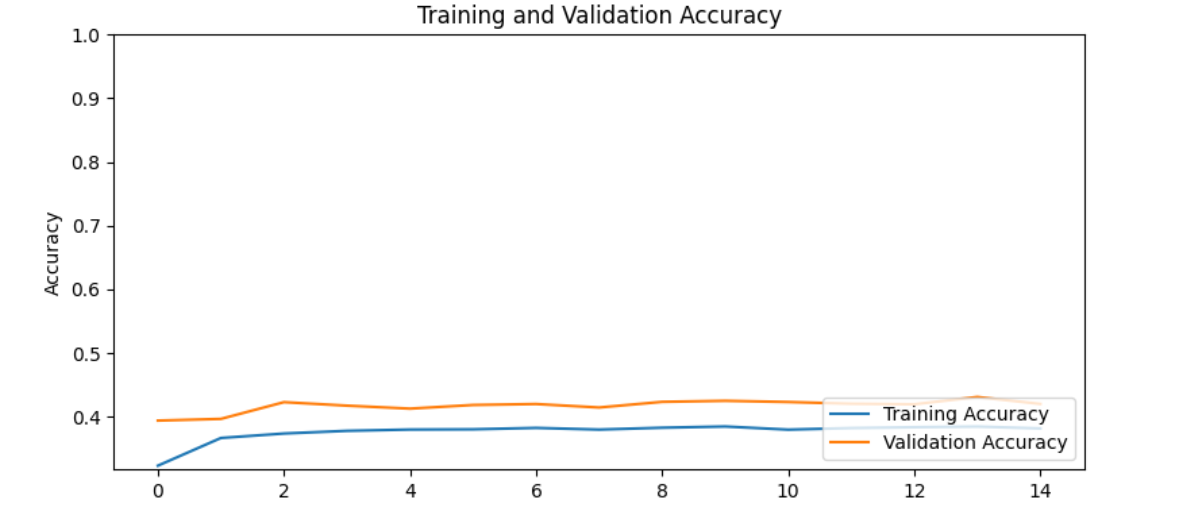
\includegraphics[width=\textwidth]{InceptionV3.png} 
    \caption{Graph of validation and training loss}
    \label{fig:InceptionV3}
\end{figure}
\subsection{Data colorization}
\label{sec:colorization}
Due to the lack of color counterparts for the grayscale images in our original dataset, we implemented a colorization algorithm based on deep learning. We used a solution published on the GeeksforGeeks \cite{gfg_colorization} portal ("Black and white image colorization with OpenCV and Deep Learning"), which is directly based on the groundbreaking 2016 research by Richard Zhang, Phillip Isola, and Alexei A. Efros from the University of California, Berkeley \cite{zhang_colorful_2016}. The foundation of this approach is a change in the way colors are represented — instead of the standard RGB model, the algorithm operates in the CIE Lab color space.
\begin{itemize}
    \item Conversion to Lab Color Space - In the first stage, the image is converted from RGB to Lab color space. The essential difference is that the Lab model completely separates brightness information from color information, whereas in the RGB model these are closely intertwined. The individual channels of the Lab color space are defined as follows:
    \begin{itemize}
        \item L: Image brightness, taking values in the range [0, 100]. In practice, this channel corresponds to a perfect grayscale photograph.
        \item a: Color axis ranging from green to red.
        \item b: Color axis ranging from blue to yellow.
    \end{itemize}
    Thanks to this separation of information, the task of the neural network is greatly simplified — it only needs to estimate the values for the a and b channels, based on the input L channel.
    \item Structure and Operation of the Convolutional Neural Network (DCNN) - The model used is a deep convolutional network implemented in the Caffe architecture. The inference process proceeds through the following steps:
   \begin{itemize}
        \item The network takes the extracted \textbf{L} channel as input, which is first rescaled to a resolution of $224 \times 224$ pixels.
        \item The image is then processed through a series of convolutional layers. Unlike classical classification networks, this architecture contains no fully connected (\texttt{Dense}) or flattening (\texttt{Flatten}) layers, which allows the spatial structure of the processed image to be preserved.
        \item Rather than treating the prediction of the \textbf{a} and \textbf{b} values as a classical regression problem (predicting continuous numerical values), the algorithm's authors reframed this as a classification problem. The network computes the probability of each pixel belonging to one of 313 predefined color variants, which are stored in the configuration file \texttt{pts\_in\_hull.npy}.
    \end{itemize}
 
    \item Fusion and Image Reconstruction - The final stage of the process is post-processing, encompassing data fusion and reconstruction of the final image. After the network generates predictions for the a and b channels, these are rescaled back to the original resolution of the input image. A fusion is then performed — the original, full-resolution L channel (derived from the source grayscale image) is combined with the AI-generated chrominance channels. By preserving the original L channel, the resulting photograph retains perfect sharpness and all the details of the original. The final step is the mathematical conversion of the reconstructed image from the CIE Lab color space back to the standard RGB color space.
\end{itemize}
Figure \ref{fig:colorized} illustrates the results of the colorization algorithm. The achieved effects are satisfactory and will enable comprehensive testing of the pre-trained models discussed in section \ref{sec:cnn_models}.

\begin{figure}[H]
    \centering
    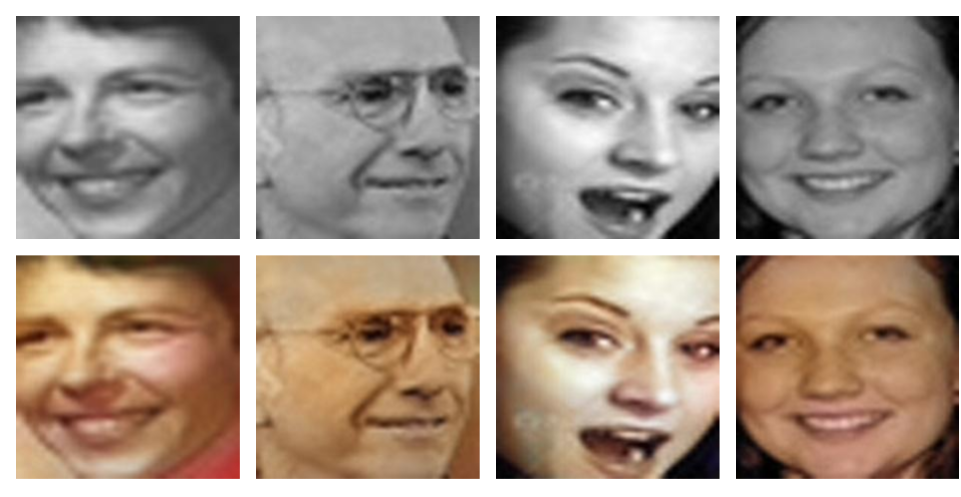
\includegraphics[width=\textwidth]{Colorized.png} 
    \caption{Photos before and after colorization}
    \label{fig:colorized}
\end{figure}
\subsection{Comparative Analysis and Final Benchmarking}
After standardizing the dataset and successfully colorizing the input images, we conducted a comprehensive evaluation of both our custom models and the pre-trained DCNN architectures. The implementation of Fine-Tuning on the pre-trained networks yielded highly visible improvements. 

As illustrated in Figure \ref{fig:vgg19_ft} and \ref{fig:resnet50_ft}, the vertical green line marks the 14th epoch, where the deeper layers of the pre-trained models were unfreezed. Immediately following this point, we observed a sharp decline in validation loss and a significant surge in accuracy. This visually confirms that the transferred representations from ImageNet successfully adapted to the facial expression domain.

\begin{figure}[H]
    \centering
    \begin{minipage}{0.48\textwidth}
        \centering
        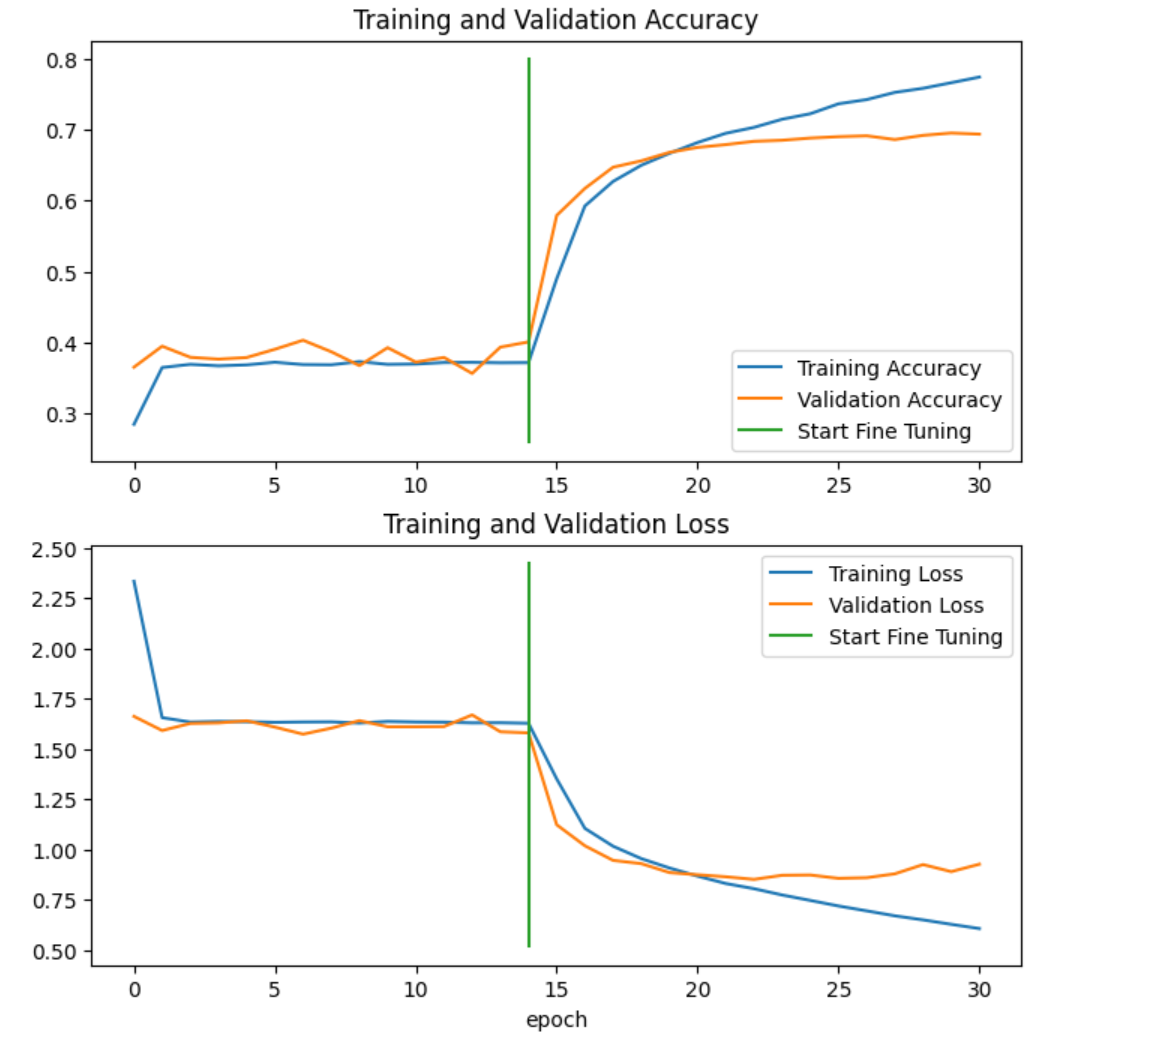
\includegraphics[width=\linewidth]{VGG19_FT.png}
        \caption{Fine-Tuning progress for VGG19}
        \label{fig:vgg19_ft}
    \end{minipage}\hfill
    \begin{minipage}{0.48\textwidth}
        \centering
        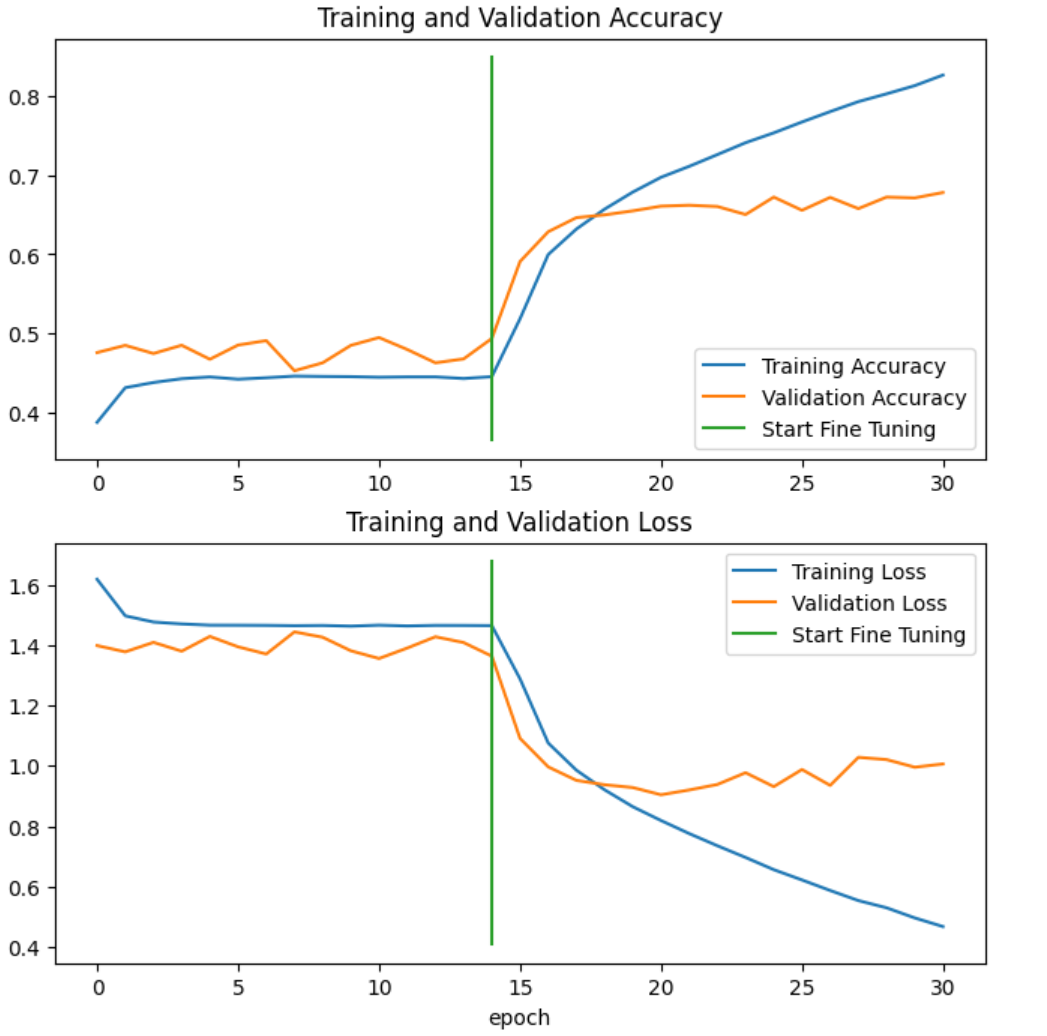
\includegraphics[width=\linewidth]{ResNet50_FT.png}
        \caption{Fine-Tuning progress for ResNet50}
        \label{fig:resnet50_ft}
    \end{minipage}
    \label{fig:ft_progress}
\end{figure}

\subsection{ConvNeXt Tiny Architecture Evaluation}
To further push the boundaries of our facial expression recognition system, we evaluated the \textbf{ConvNeXt Tiny} architecture. Unlike the fine-tuning strategy employed for the VGG and ResNet models, where only the top 20\% of layers were unfrozen, the ConvNeXt Tiny training utilized a more aggressive, two-phase approach.

The model was built with a frozen ImageNet-pretrained base, followed by a custom classification head consisting of a Global Average Pooling 2D layer, Batch Normalization, Dropout (set to 0.4 for strong regularization), and two Dense layers (256 neurons with ReLU and 7 neurons with Softmax).

\begin{itemize}
    \item \textbf{Phase 1 (Warm-up):} The custom head was trained exclusively for 5 epochs with a standard learning rate ($1 \times 10^{-3}$) to initialize the classification weights.
    \item \textbf{Phase 2 (Fine-Tuning):} The entire ConvNeXt base model was unfrozen. A substantially reduced learning rate of $1 \times 10^{-5}$ was applied to carefully adjust the deep convolutional weights without destroying the valuable representations learned on the ImageNet dataset.
\end{itemize}

During our experimental runs, we encountered significant environmental instability. The first trial was scheduled for 20 epochs. After approximately 12 hours of training, the kernel crashed at epoch 15 due to memory exhaustion. Despite the abrupt termination, the model recorded an impressive peak validation accuracy of \textbf{74.56\%} and an estimated macro-precision of approximately \textbf{73.55\%}. 

To ensure stability and secure a fully completed training cycle, a second run was executed with a reduced target of 10 epochs. This run successfully finished, achieving a validation accuracy of \textbf{73.60\%} and a macro-precision of \textbf{72.64\%}. 

Both ConvNeXt Tiny trials successfully surpassed our previous top-performing custom \texttt{second\_model}, which had previously achieved the highest classification accuracy at 71.04\%.

The comparative analysis of all tested architectures, now including the ConvNeXt Tiny iterations, is compiled in Table \ref{tab:final_results}.

\begin{table}[H]
    \centering
    \begin{tabular}{|l|c|c|}
        \hline
        \textbf{Model} & \textbf{Accuracy} & \textbf{Macro-Precision} \\
\hline
        ConvNeXt Tiny (15 epochs - crashed) & \textbf{74.56\%} & \textbf{$\sim$73.55\%} \\
        ConvNeXt Tiny (10 epochs - completed) & \textbf{73.60\%} & \textbf{72.64\%} \\
        second\_model & 71.04\% & 70.19\% \\
        VGG19 & 70.07\% & 69.47\% \\
        VGG16 & 68.24\% & 66.57\% \\
        ResNet50 & 68.00\% & 67.40\% \\
        third\_model & 67.81\% & 66.42\% \\
        ResNet101 & 67.71\% & 66.87\% \\
        InceptionV3 & 62.15\% & 60.84\% \\
        first\_model & 56.17\% & 54.03\% \\
        \hline
    \end{tabular}
    \caption{Final comparison of model performance metrics}
    \label{tab:final_results}
\end{table}

he confusion matrix for the completed ConvNeXt Tiny training session (10 epochs) is presented in Figure \ref{fig:cm_convnext}. 

\begin{figure}[H]
    \centering
    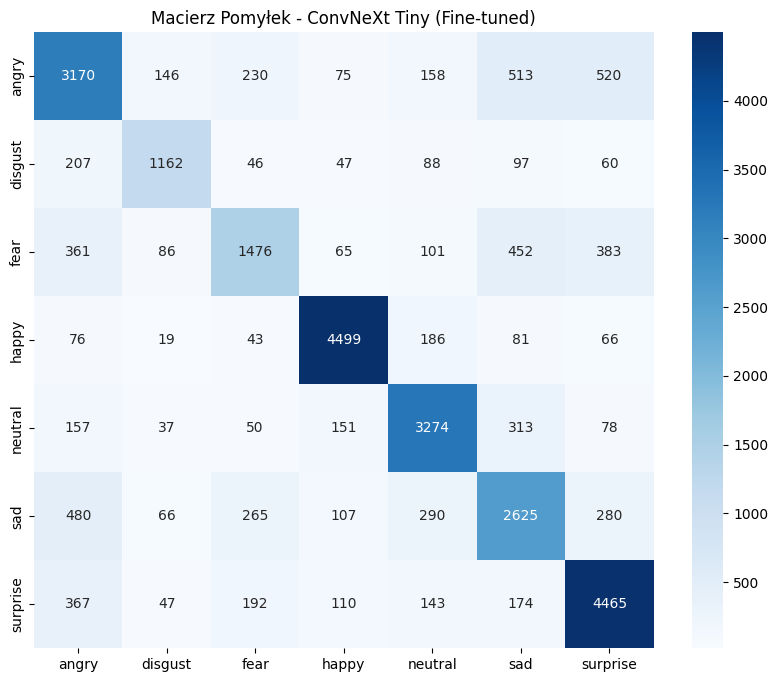
\includegraphics[width=\textwidth]{convnext_cm.png} 
    \caption{Confusion Matrix - ConvNeXt Tiny (Fine-tuned, 10 epochs)}
    \label{fig:cm_convnext}
\end{figure}

The matrix reveals that the model significantly improved recognition across difficult categories, particularly in distinguishing between "sad" and "neutral" states, which was a known bottleneck in previous architectures like the \texttt{second\_model}. This success is attributed to the combination of the modern ConvNeXt architecture and the two-stage fine-tuning process, where the entire base was eventually unfrozen to adapt to facial features. 

The high macro-precision of 72.64\% confirms that the model is not just biased toward the most frequent classes but maintains a high level of reliability across all seven emotional states. This makes it the most suitable candidate for deployment on the target hardware platform (Raspberry Pi), despite its higher computational requirements compared to the initial basic models.

\section{Real-Time Face Detection and Recognition System}
To ensure the robotic head can interact dynamically with its environment, a real-time vision processing subsystem was implemented. During the development phase, two distinct architectural approaches were tested to evaluate performance, accuracy, and resource utilization: a CPU-based system utilizing HOG (Histogram of Oriented Gradients) and a GPU-accelerated system leveraging the InsightFace framework.

\subsection{CPU-Based Approach (HOG)}
The initial prototype was designed to run entirely on the CPU using the \texttt{face\_recognition} library, which relies on dlib's state-of-the-art C++ toolkit. 
\begin{itemize}
    \item \textbf{Detection Algorithm:} Histogram of Oriented Gradients (HOG) combined with a linear classifier.
    \item \textbf{Implementation Details:} To maintain a functional framerate, the input video stream was downscaled by a factor of 4 (scale factor = 0.25). 
    \item \textbf{Pros \& Cons:} While highly accessible and requiring no specialized hardware or CUDA configuration, the CPU-bound approach struggles with high-resolution frames and multiple faces, leading to significant thermal throttling and lower FPS.
\end{itemize}

\subsection{GPU-Accelerated Approach (InsightFace)}
To overcome the computational bottlenecks, the system was migrated to a GPU-accelerated architecture using the \texttt{InsightFace} library with the ONNX Runtime (CUDA Execution Provider).
\begin{itemize}
    \item \textbf{Detection Algorithm:} Deep neural networks optimized for spatial detection and feature extraction.
    \item \textbf{Implementation Details:} This script processes a designated "active zone" in the center of the frame to minimize unnecessary computation. It integrates directly with the trained Keras emotion classification model, analyzing frames at regular intervals (\texttt{EMOTION\_SKIP\_FRAMES = 3}) to balance accuracy and performance. Face data and emotional states are serialized to a JSON file for the conversation subsystem.
    \item \textbf{Pros \& Cons:} This approach offloads heavy matrix multiplications to the GPU, allowing for processing of higher resolution frames (up to 720p) with minimal CPU overhead.
\end{itemize}

\subsection{Hardware Performance Comparison}
Benchmarking was conducted to quantify the performance delta between the two implementations across various hardware configurations. The tests compare legacy CPU-bound methods (HOG) with modern GPU acceleration (InsightFace).

\begin{itemize}
    \item \textbf{Setup A (Main Workstation):}
    \begin{itemize}
        \item CPU: Intel Core i5-10400F (2.90 GHz)
        \item GPU: NVIDIA GeForce GTX 1060 (6GB GDDR5)
    \end{itemize}
    
    \item \textbf{Setup B (Mobile Workstation):}
    \begin{itemize}
        \item CPU: 12th Gen Intel Core i5-12450H (2.00 GHz)
        \item GPU: NVIDIA GeForce RTX 3050Ti (4GB GDDR6)
    \end{itemize}

    \item \textbf{Setup C (High-End Mobile Workstation):}
    \begin{itemize}
        \item CPU: Intel Core i9-13900HX (2.20 GHz)
        \item GPU: NVIDIA GeForce RTX 4060 (8GB GDDR6)
    \end{itemize}

    \item \textbf{Setup D (Target Platform - Raspberry Pi 5):}
    \begin{itemize}
        \item CPU: Broadcom BCM2712 (ARM v8) @ 2.4GHz
        \item RAM: 8GB LPDDR4X
    \end{itemize}
\end{itemize}

\subsubsection{CPU-Based Performance (HOG)}
The following table summarizes the performance of the HOG-based detection algorithm. FPS values increase significantly when no face is present due to the bypass of embedding and emotion classification models.

\begin{table}[H]
    \centering
    \begin{tabular}{|l|c|c|}
        \hline
        \textbf{Hardware Setup} & \textbf{Face Detected} & \textbf{No Face Detected} \\
        \hline
        Setup A (GTX 1060 / i5-10400F) & 2-3 FPS & 40-50 FPS \\
        Setup B (RTX 3050Ti / i5-12450H) & 3-4 FPS & 50-60 FPS \\
        Setup C (RTX 4060 / i9-13900HX) & 4 FPS & 90 FPS \\
        Setup D (Raspberry Pi 5) & N/A & N/A \\
        \hline
    \end{tabular}
    \caption{Performance results for CPU-based HOG detection.}
    \label{tab:fps_hog}
\end{table}

\subsubsection{GPU-Accelerated Performance (InsightFace)}
The GPU-based approach offloads heavy matrix multiplications, enabling higher efficiency.

\begin{table}[H]
    \centering
    \begin{tabular}{|l|c|c|}
        \hline
        \textbf{Hardware Setup} & \textbf{Face Detected} & \textbf{No Face Detected} \\
        \hline
        Setup A (GTX 1060 / i5-10400F) & 22-26 FPS & 35-45 FPS \\
        Setup B (RTX 3050Ti / i5-12450H) & 20-25 FPS & 35-45 FPS \\
        Setup C (RTX 4060 / i9-13900HX) & 30-35 FPS & 65-70 FPS \\
        Setup D (Raspberry Pi 5) & N/A & N/A \\
        \hline
    \end{tabular}
    \caption{Performance results for GPU-accelerated InsightFace detection.}
    \label{tab:fps_insightface}
\end{table}

\subsubsection{Raspberry Pi 5 Performance Profiling (Target Platform)}
To thoroughly evaluate the system's behavior on the target hardware (Setup D), a series of stress tests were conducted using the \texttt{btop} resource monitor. The profiling focused on CPU utilization, memory footprint, and thermal performance during two distinct states: idling (no face in the frame) and active processing (face detected, invoking face recognition and emotion classification models).

\paragraph{HOG-Based Implementation}
The CPU-bound approach utilizing Histogram of Oriented Gradients (HOG) demonstrated highly variable resource consumption depending on the system state.

\begin{figure}[H]
    \centering
    \begin{minipage}{0.48\textwidth}
        \centering
        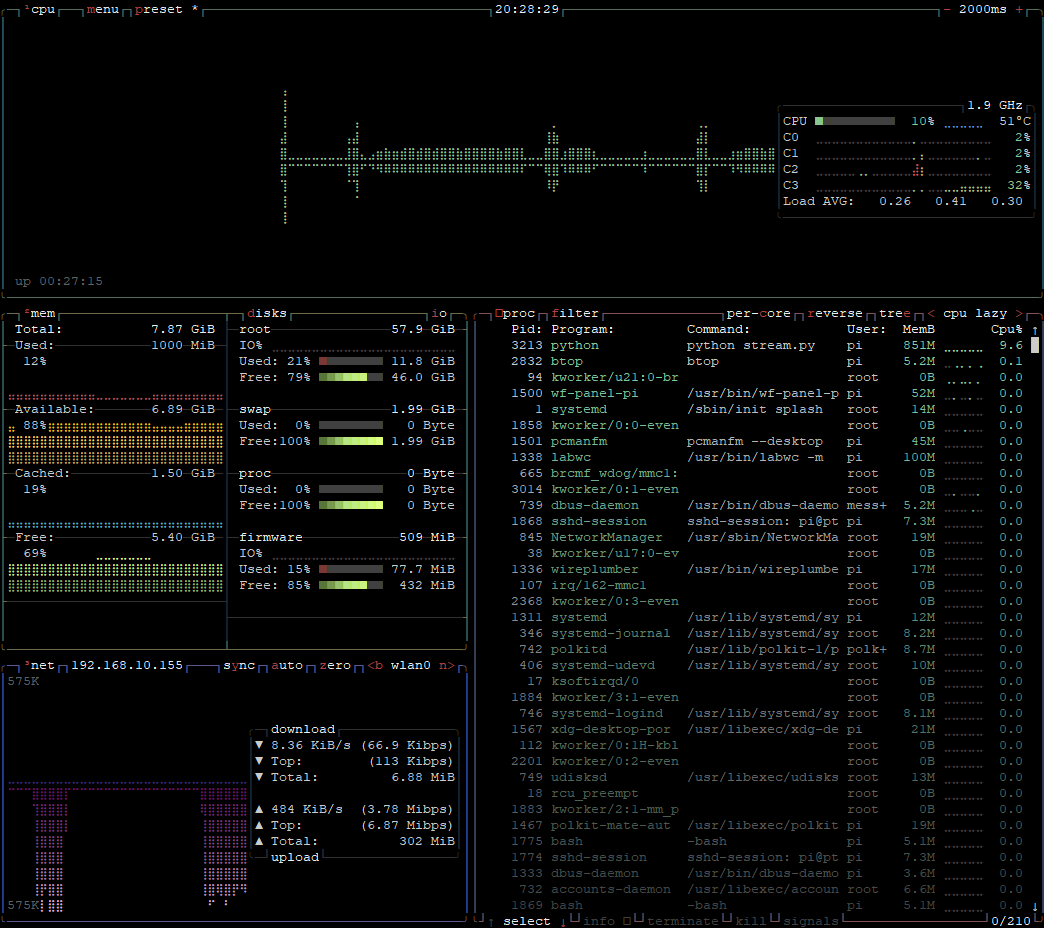
\includegraphics[width=\linewidth]{hogt_without_face.png}
        \caption{HOG - Idle state (No face)}
        \label{fig:hog_idle}
    \end{minipage}\hfill
    \begin{minipage}{0.48\textwidth}
        \centering
        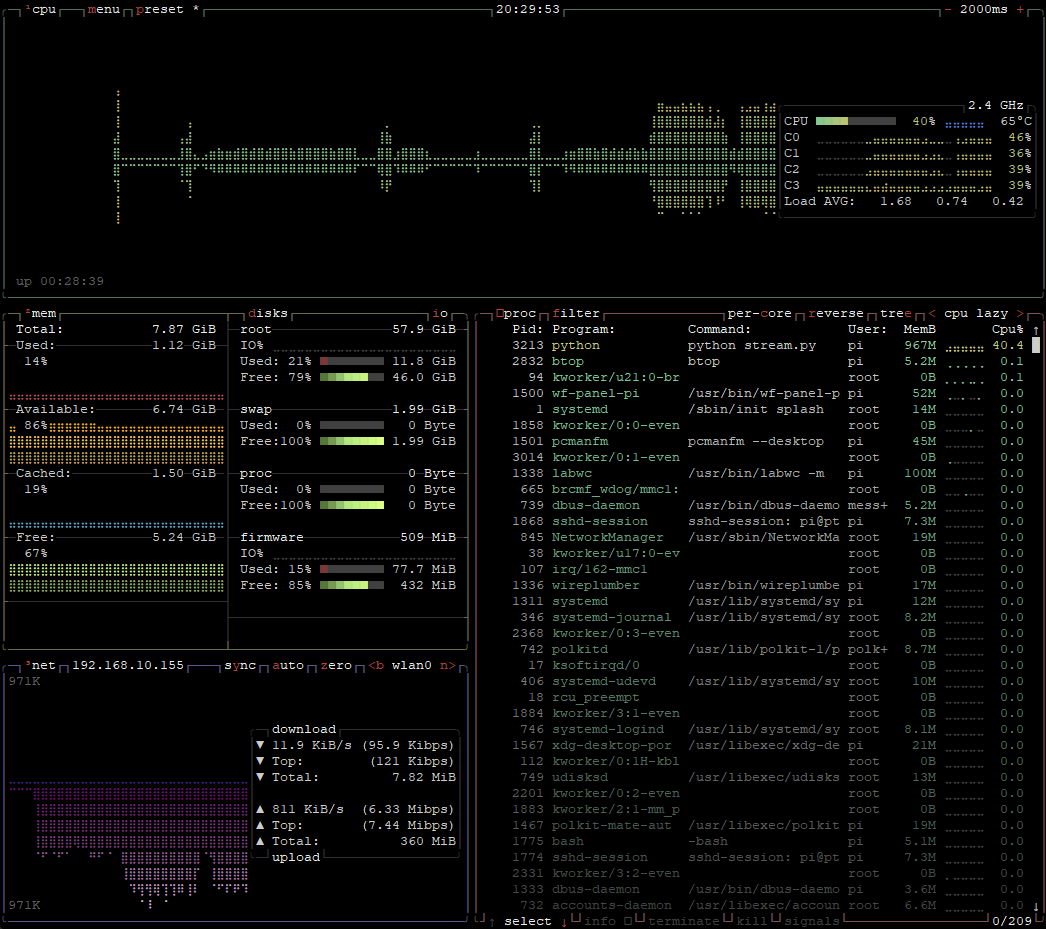
\includegraphics[width=\linewidth]{hogt_with_face.png}
        \caption{HOG - Active state (Face detected)}
        \label{fig:hog_active}
    \end{minipage}
\end{figure}

As observed in Figures \ref{fig:hog_idle} and \ref{fig:hog_active}, when no face is present, the system remains exceptionally cool (51$^{\circ}$C) with minimal CPU utilization (approximately 10\%). However, upon face detection, total CPU load increases to roughly 40\%, and the temperature stabilizes at 65$^{\circ}$C. This moderate total load suggests that the \texttt{dlib} backend is constrained by single-thread performance bottlenecks and cannot fully saturate all four cores of the Raspberry Pi 5. Memory usage remains stable at approximately 1.1 GB.

\paragraph{YuNet-Based Implementation}
The OpenCV-accelerated YuNet model, while offering superior detection accuracy and framerate scalability, exhibits a significantly more aggressive hardware footprint on the ARM architecture.

\begin{figure}[H]
    \centering
    \begin{minipage}{0.48\textwidth}
        \centering
        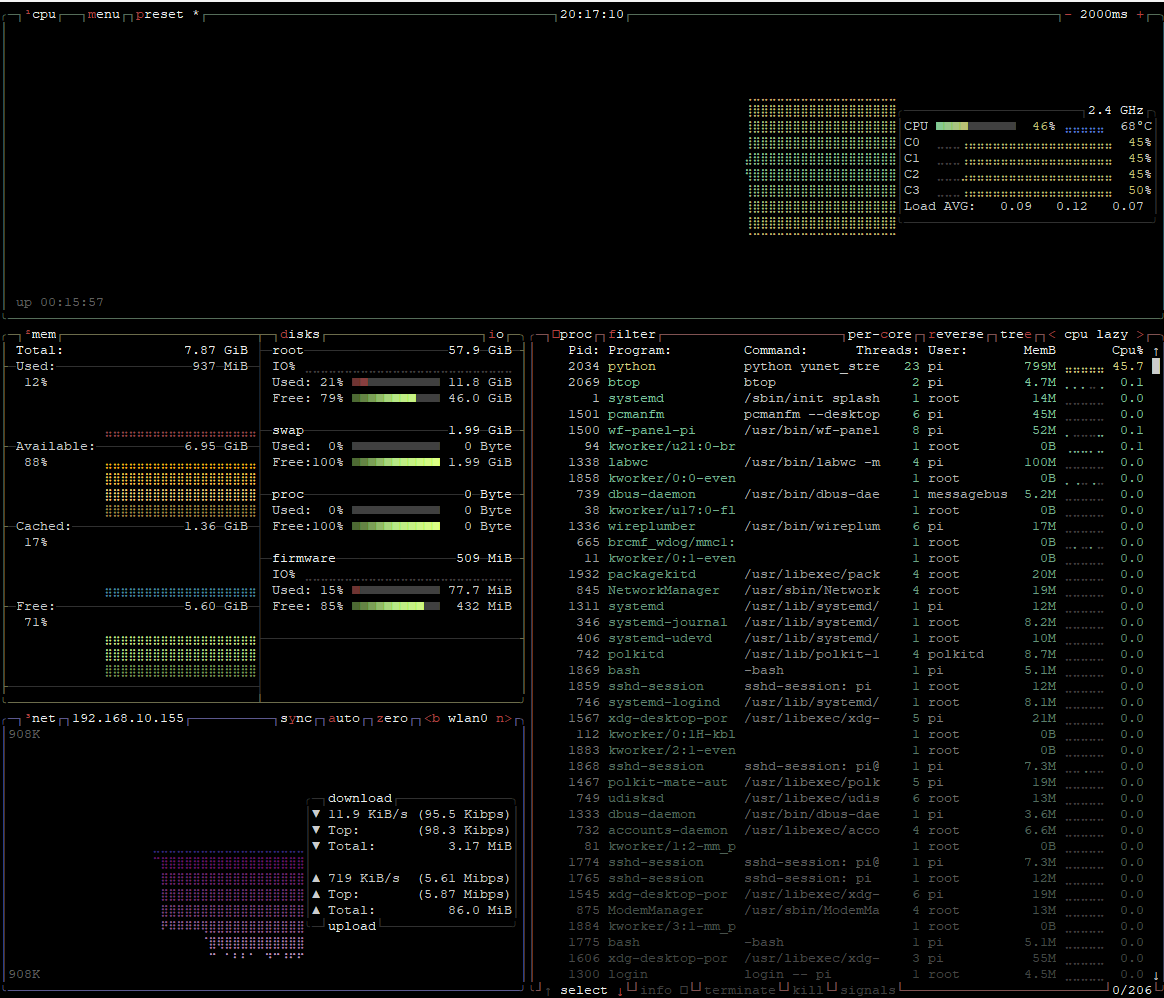
\includegraphics[width=\linewidth]{yunet_without_face.png}
        \caption{YuNet - Idle state (No face)}
        \label{fig:yunet_idle}
    \end{minipage}\hfill
    \begin{minipage}{0.48\textwidth}
        \centering
        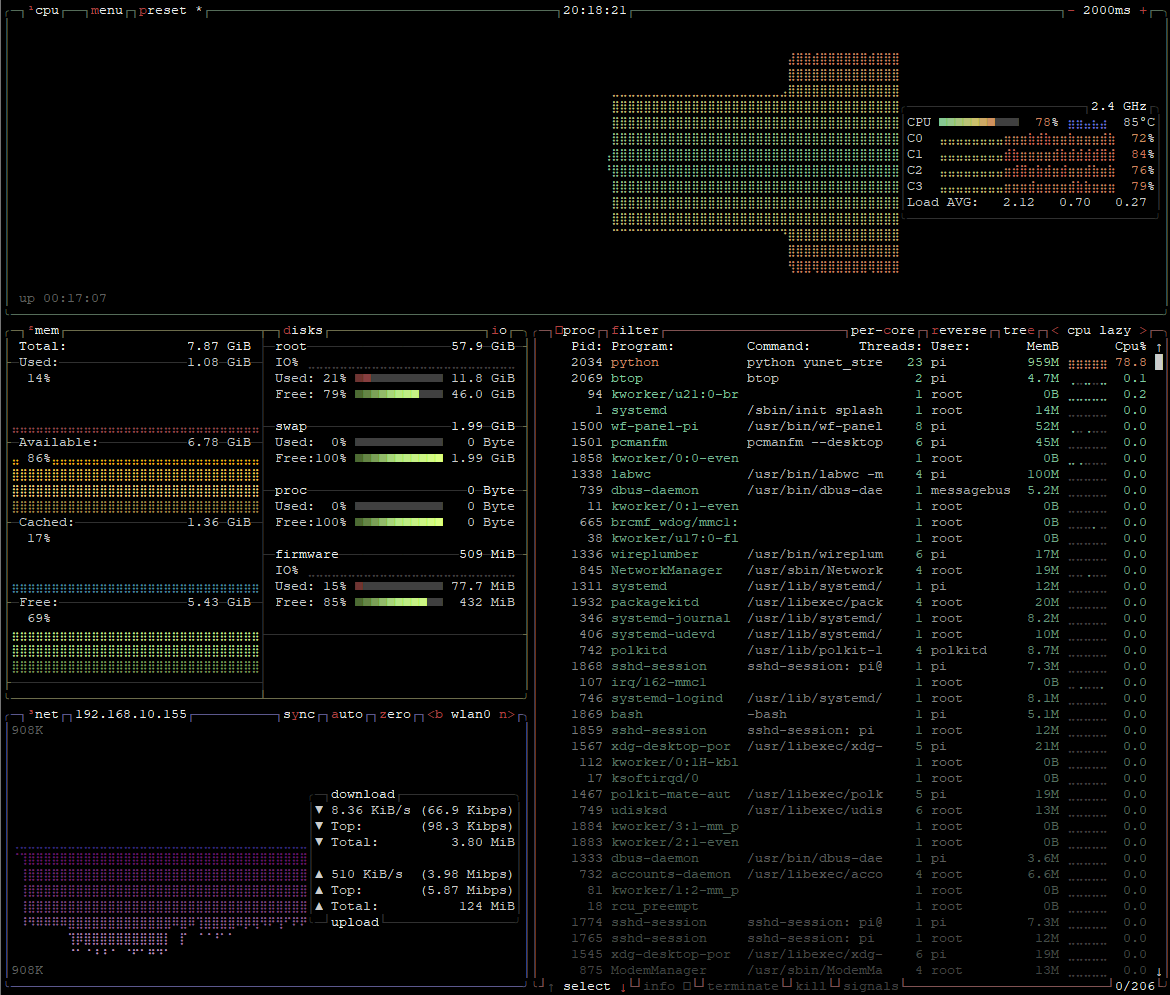
\includegraphics[width=\linewidth]{yunet_with_face.png}
        \caption{YuNet - Active state (Face detected)}
        \label{fig:yunet_active}
    \end{minipage}
\end{figure}

Figures \ref{fig:yunet_idle} and \ref{fig:yunet_active} illustrate a high baseline operational cost. Even without a face in the frame, continuous neural network inference consumes roughly 46\% of total CPU capacity, elevating the temperature to 68$^{\circ}$C. During active face tracking and emotion recognition, the highly parallelized nature of the OpenCV DNN module heavily tasks the processor, driving total CPU utilization to nearly 79\%. 

Consequently, the SoC temperature reaches 85$^{\circ}$C. This is a critical threshold for the Broadcom BCM2712 chip, at which aggressive thermal throttling occurs, severely degrading performance. These results unequivocally demonstrate that deploying the robust YuNet pipeline on the Raspberry Pi 5 strictly mandates a dedicated active cooling solution (e.g., the official Raspberry Pi Active Cooler) to maintain system stability and real-time processing capabilities over prolonged interaction periods.

\subsubsection{Performance with Active Cooler (Radiator)}
To verify the hypothesis regarding the necessity of active cooling, the stress tests were repeated with an official Raspberry Pi Active Cooler attached to the SoC. The results confirmed that the cooling solution effectively eliminates the thermal throttling problem for both implementations.

\paragraph{HOG-Based Implementation with Active Cooler}

\begin{figure}[H]
    \centering
    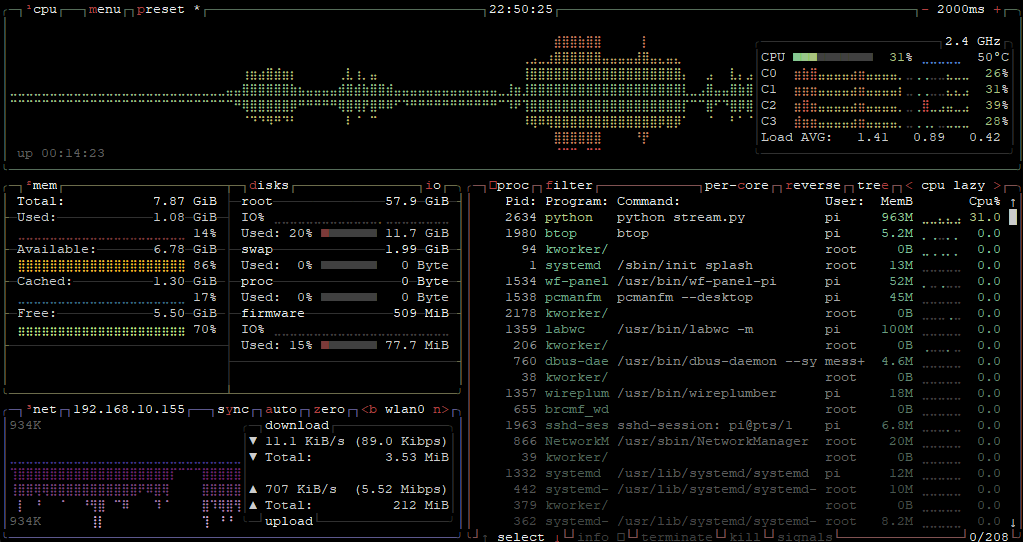
\includegraphics[width=0.75\linewidth]{hog_with_radiator.png}
    \caption{HOG - Active state (Face detected) with Active Cooler}
    \label{fig:hog_radiator}
\end{figure}

As shown in Figure~\ref{fig:hog_radiator}, with the active cooler attached, the HOG-based pipeline running in full face-detection mode (process \texttt{python stream.py} visible at the top of the process list) operates with a total CPU load of approximately 31\% and a SoC temperature of only 50$^{\circ}$C. This represents a substantial thermal improvement compared to the uncooled scenario (65$^{\circ}$C under the same workload), confirming that the cooler effectively dissipates the heat generated by the dlib-based pipeline. Memory consumption remains stable at approximately 1.08~GB.

\paragraph{YuNet-Based Implementation with Active Cooler}

\begin{figure}[H]
    \centering
    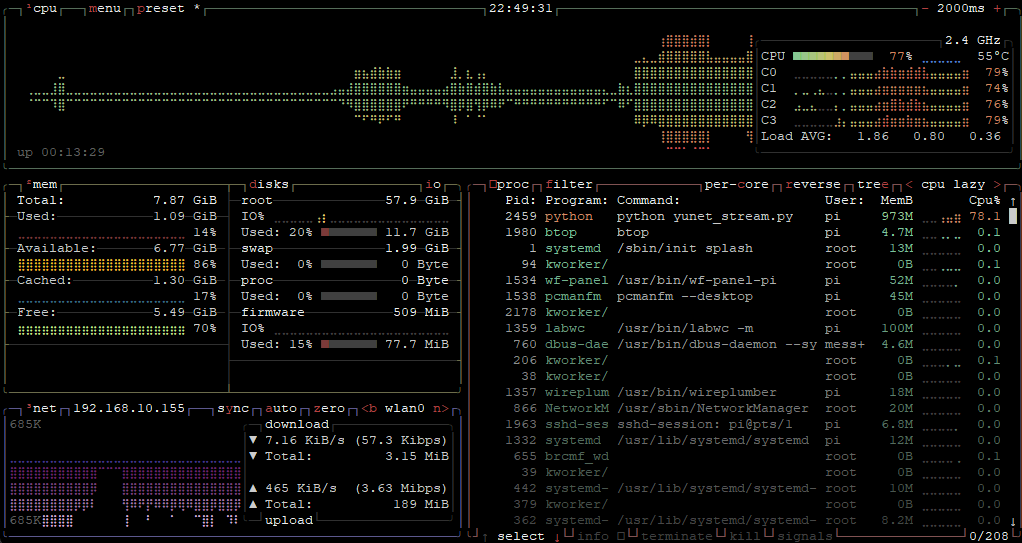
\includegraphics[width=0.75\linewidth]{yunet_with_radiator.png}
    \caption{YuNet - Active state (Face detected) with Active Cooler}
    \label{fig:yunet_radiator}
\end{figure}

Figure~\ref{fig:yunet_radiator} illustrates the thermal impact of the active cooler on the more demanding YuNet pipeline. With \texttt{python yunet\_stream.py} consuming approximately 78\% of a single core and the overall CPU utilization reaching 77\%, the SoC temperature is held at 55$^{\circ}$C — a dramatic reduction from the critical 85$^{\circ}$C recorded without cooling. This result demonstrates that the active cooler is fully capable of sustaining the YuNet workload within safe thermal boundaries indefinitely, without triggering throttling. Memory usage remains stable at approximately 1.09~GB.

\paragraph{Summary}
The introduction of the active cooler reduces peak SoC temperatures by 15$^{\circ}$C for the HOG pipeline and by 30$^{\circ}$C for the YuNet pipeline. These findings confirm that the Raspberry Pi Active Cooler is a mandatory hardware component for any deployment of the vision module in a sustained, real-time interaction scenario — particularly when using the OpenCV DNN-accelerated YuNet backend.

\subsection{Finalized Vision Pipeline: YuNet and SFace Integration}
To achieve the optimal balance between high framerates on the Raspberry Pi 5 and reliable recognition, the final production pipeline was built around OpenCV's YuNet for face detection and SFace for facial recognition. This approach bypasses the heavy overhead of previous methods while maintaining robust accuracy.

\textbf{Detection and Recognition Flow} \\
The system continuously captures frames using Picamera2. YuNet efficiently isolates the largest face in the frame, which is then cropped and aligned. The SFace model extracts a 128-dimensional feature vector (embedding) from this crop. Recognition is performed by calculating the cosine similarity against known vectors stored in the local database, with a strict matching threshold set to 0.28.

\textbf{Pipeline Stabilization and Logic} \\
To ensure smooth operation and steady tracking, the pipeline integrates a rolling buffer (majority voting) for identity confirmation and triggers the heavy emotion classification model strictly on an event-driven basis (only when a new identity is confirmed or a session starts). 

\section{Inter-Module Communication}
The vision system operates as an independent network component communicating with the natural language processing module using a client-server architecture based on the Flask framework. The Raspberry Pi runs a local web server that serves a dual role.

On one hand, it continuously broadcasts a video stream and sends telemetry packets containing frame coordinates, user ID, and the recognized emotional state directly to the external master module. Data transmission is handled via network requests, ensuring full compatibility across different programming environments.

On the other hand, the server listens for incoming requests. When the master system recognizes a new name during voice interaction or issues a command to change facial expressions, it sends a corresponding return packet. The server on the microcomputer receives this information via endpoints for new users and for lip control, immediately passing it to the internal program layers responsible for database updates and robot behavior modification.

\section{Technical Challenges and Optimization}
Building a real-time vision system on embedded hardware introduced several constraints that required specific architectural solutions.

The Raspberry Pi 5 provides significant computational power, but high-intensity neural network inference leads to rapid heat accumulation. During initial tests, the SoC temperature reached a critical threshold of 85 degrees Celsius, causing thermal throttling. The implementation of an active cooling solution was necessary to maintain a stable clock speed and prevent system degradation during prolonged operation.

Initially, running the complex emotion classification model on every single frame proved to be a major bottleneck, resulting in poor performance of only 4-5 FPS. To address this, we transitioned to an event-driven architecture where the emotion network is triggered only upon a confirmed identity change or at the start of a new session. This optimization allowed the system to maintain a much smoother and more responsive performance of 14-15 FPS. To further improve reliability, we implemented a majority voting filter using a rolling buffer of seven frames to eliminate identity flickering caused by lighting shifts.

A major challenge was the gap between synthetic training data and real-world performance. While Flux.1 generated visually perfect images, models trained exclusively on these samples failed to generalize to actual camera feeds. We resolved this by modifying the generation prompts to include realistic noise and varied lighting, which provided the necessary variance for practical deployment.

\section{Data Privacy and Security}
The vision module was designed with strict privacy protection principles in mind. The system architecture completely excludes storing raw image files or video recordings on the device's drive. Every detected face is immediately transformed into a digital feature vector, which is a 128-dimensional set of numbers describing facial geometry, from which it is impossible to reconstruct the original human image. This data is stored in a local SQLite database.

To optimize disk space and maintain data security, an automated profile lifecycle was introduced. Upon each startup, the system checks timestamps and irrevocably deletes entries older than seven days. Additionally, the database has a strict capacity limit set to 200 profiles. If this value is exceeded, the defense mechanism automatically purges the oldest records, making room for new users and preventing memory overflow.

\section{Conception and tests new model}
This part of the project focused on designing and evaluating a new approach for a Facial Emotion Recognition (FER) system. Rather than relying on a standard single network analyzing the entire frame, the new approach assumes the deployment of a multi-stage processing pipeline based on cascaded CNN networks.

\subsection{Solution Architecture}
The solution architecture consists of two main modules:

\begin{itemize}
    \item Feature Extraction Module: The first stage is a CNN model serving as a precise Region of Interest (ROI) detector. Its task is to extract the key facial components of the user, specifically: eyebrows, eyes, and mouth.
    \item Final Classification Module: The segmented components are then passed to the target neural network. Its task is to analyze the spatial relationships and shape of only those isolated facial features in order to make a final prediction across one of 7 classes (6 basic emotions + neutral state).
\end{itemize}

\subsection{Benefits of This Approach}
\begin{itemize}
    \item Increased accuracy: Initial research indicates that the cascaded approach enables higher detection precision. The main classifier focuses exclusively on "clean" facial expression signals, rather than wasting computational resources on analyzing irrelevant details in the image.
    \item Greater robustness to noise: The system becomes significantly less susceptible to variable environmental conditions (such as lighting, background, or the user's hairstyle), since the decision-making process relies strictly on isolated facial components.
\end{itemize}

\subsection{Training Data Strategy (Dataset)}
To provide the model with optimal conditions for generalization and to avoid overfitting, a comprehensive dataset has been designed:

\begin{itemize}
    \item Volume: The dataset will consist of 49,000 images in total, ensuring perfect class balance (exactly 7,000 samples per each of the 7 emotions analyzed).
    \item Demographic diversity: The dataset has been planned with careful attention to the absence of bias, and will therefore be diverse in terms of ethnicity and age.
    \item Synthetic augmentation (Generative Augmentation): Due to the difficulty in acquiring such a large number of balanced, real-world, high-quality images, at least half of the dataset will be generated synthetically using the advanced diffusion model flux2.dev. This will allow for controlled creation of edge cases and precise management of the demographics of the generated faces.
\end{itemize}

\section{Conclusion}
The development of the vision module for the robotic head successfully met its primary objectives. Through rigorous data preprocessing, including pHash deduplication, OCR artifact removal, demographic filtering, and data augmentation via Generative AI (Flux.1), we constructed a highly robust training corpus of over 120,000 images.

The comparative study between custom-designed Convolutional Neural Networks and industry-standard transfer learning models (VGG, ResNet, Inception, ConvNeXt) yielded highly satisfactory results. While our custom \texttt{second\_model} achieved a highly commendable accuracy of 71.04\%, closely approaching our initial 75\% target, the integration of the ConvNeXt Tiny architecture pushed our results even further, peaking at 74.56\%.

The application of Fine-Tuning and innovative data colorization techniques proved highly effective. While heavy architectures like ResNet101 and InceptionV3 did not justify their computational overhead in this specific use case, modern architectures like ConvNeXt Tiny demonstrate immense potential. The best-performing models will serve as a reliable engine to feed affective data to the robot's speech synthesis subsystem, paving the way for empathetic, human-robot interaction.
\begin{thebibliography}{9}

    \bibitem{blazeface} 
    V. Bazarevsky, Y. Kartynnik, A. Vakunov, K. Raveendran, i M. Grundmann, „BlazeFace: Sub-millisecond Neural Face Detection on Mobile GPUs”, arXiv preprint arXiv:1907.05047, 2019. \href{https://arxiv.org/abs/1907.05047}{[Link to the article]} 
    
    \bibitem{mediapipe} 
    C. Lugaresi et al., „MediaPipe: A Framework for Building Perception Pipelines”, arXiv preprint arXiv:1906.08172, 2019. \href{https://arxiv.org/abs/1906.08172}{[Link to the article]} 
    
    \bibitem{tensorflow} 
    M. Abadi et al., „TensorFlow: Large-Scale Machine Learning on Heterogeneous Distributed Systems”, arXiv preprint arXiv:1603.04467, 2016. \href{https://www.tensorflow.org/}{[Link to the article]} 
    \bibitem{fer2013}
    (fer2013+affectnet) dataset - Emotions - found on kaggle site form user PrasadSomvanshi on license Apache 2.0 \href{https://www.kaggle.com/datasets/prasadsomvanshih/fer2013-affectnet-dataset-emotions/data?fbclid=IwY2xjawQOZipleHRuA2FlbQIxMQBzcnRjBmFwcF9pZAEwAAEeeakwhP0rBKTNC9dH0_7OUlwZgdrUVN_qAnQQVBijJ42LuroL_KM-VX6xPaM_aem_M1YE76_0EMbx7yb1aUcGzQ}{link to dataset}
    \bibitem{affect}
    Facial Affect Dataset Balanced - found on kaggle site from user Viktor Modroczký on license Attribution-NonCommercial-ShareAlike 3.0 IGO (CC BY-NC-SA 3.0 IGO) \href{https://www.kaggle.com/datasets/viktormodroczky/facial-affect-dataset}{link to the dataset}
    \bibitem{Humman face emotions}
    Human Face Emotions - found on kaggle site from user Samith Chimminiyan on License Apache 2.0 \href{https://www.kaggle.com/datasets/samithsachidanandan/human-face-emotions?fbclid=IwY2xjawQRS4pleHRuA2FlbQIxMQBzcnRjBmFwcF9pZAEwAAEeFoE2tKxAJHbQbfM4sPKdUYLckVtJX8uKNkO-qEWGZ1SNsIFSDW6J9IakJq8_aem_CrDZH0whQgTOAbaWuiPq2w}{link to the dataset}
    \bibitem{Facial Emotion Recognition Dataset}
    Facial Emotion Recognition Dataset - found on kaggle site from user FahadullahA on license: Attribution 4.0 International (CC BY 4.0) \href{https://www.kaggle.com/datasets/fahadullaha/facial-emotion-recognition-dataset?fbclid=IwY2xjawQRS4xleHRuA2FlbQIxMQBzcnRjBmFwcF9pZAEwAAEeNf73G1bYjDj_hAsEGtd7YcKzrPsfmEE5SWb8qHwRVCud6sVvNcniatFb4Ac_aem_A_MxoTH_SaY2XDt-hgU_7Q}{link to the dataset}
    \bibitem{emonetface2025} 
    C. Schuhmann et al., „EmoNet-Face: An Expert-Annotated Benchmark for Synthetic Emotion Recognition”, arXiv preprint arXiv:2505.20033, 2025. \href{https://arxiv.org/abs/2505.20033}{[Link to the article]}
    \bibitem{expw} 
    Markson14, „ExpWCleaned Dataset - Emotion Recognition in the Wild”, GitHub Repository, \href{https://github.com/markson14/ExpWCleaned}{[Link to dataset]} 
    \bibitem{flux}
    Black Forest Labs, \textit{FLUX.1-dev}, Hugging Face, 2024. 
    \href{https://huggingface.co/black-forest-labs/FLUX.1-dev}{Link to the model}.
    \bibitem{inceptionv3} 
    C. Szegedy, V. Vanhoucke, S. Ioffe, J. Shlens, i Z. Wojna, „Rethinking the Inception Architecture for Computer Vision”, w: \textit{Proceedings of the IEEE Conference on Computer Vision and Pattern Recognition (CVPR)}, 2016, s. 2818-2826. \href{https://arxiv.org/abs/1512.00567}{[Link to the article]}
    
    \bibitem{resnet} 
    K. He, X. Zhang, S. Ren, i J. Sun, „Deep Residual Learning for Image Recognition”, w: \textit{Proceedings of the IEEE Conference on Computer Vision and Pattern Recognition (CVPR)}, 2016, s. 770-778. \href{https://arxiv.org/abs/1512.03385}{[Link to the article]}
    
    \bibitem{vgg} 
    K. Simonyan i A. Zisserman, „Very Deep Convolutional Networks for Large-Scale Image Recognition”, \textit{arXiv preprint arXiv:1409.1556}, 2014. \href{https://arxiv.org/abs/1409.1556}{[Link to the article]}
    
    \bibitem{xception} 
    F. Chollet, „Xception: Deep Learning with Depthwise Separable Convolutions”, w: \textit{Proceedings of the IEEE Conference on Computer Vision and Pattern Recognition (CVPR)}, 2017, s. 1251-1258. \href{https://arxiv.org/abs/1610.02357}{[Link to the article]}
    \bibitem{zhang_colorful_2016}
    R. Zhang, P. Isola, and A. A. Efros, ``Colorful Image Colorization'', in \textit{European Conference on Computer Vision (ECCV)}, Springer, 2016, pp. 649--666. \href{https://arxiv.org/abs/1603.08511}{[Link to the paper]}
    \bibitem{gfg_colorization}
    GeeksforGeeks, ``Black and white image colorization with OpenCV and Deep Learning''. Available at: \href{https://www.geeksforgeeks.org/computer-vision/black-and-white-image-colorization-with-opencv-and-deep-learning/}{[Link to the article]} (Accessed: March 13, 2026).
    
\end{thebibliography}
\end{document}